\documentclass[12pt,]{article}
\usepackage[left=1in,top=1in,right=1in,bottom=1in]{geometry}
\newcommand*{\authorfont}{\fontfamily{phv}\selectfont}
\usepackage{lmodern}


  \usepackage[T1]{fontenc}
  \usepackage[utf8]{inputenc}



\usepackage{abstract}
\renewcommand{\abstractname}{}    % clear the title
\renewcommand{\absnamepos}{empty} % originally center

\renewenvironment{abstract}
 {{%
    \setlength{\leftmargin}{0mm}
    \setlength{\rightmargin}{\leftmargin}%
  }%
  \relax}
 {\endlist}

\makeatletter
\def\@maketitle{%
  \newpage
%  \null
%  \vskip 2em%
%  \begin{center}%
  \let \footnote \thanks
    {\fontsize{18}{20}\selectfont\raggedright  \setlength{\parindent}{0pt} \@title \par}%
}
%\fi
\makeatother




\setcounter{secnumdepth}{0}

\usepackage{caption}
\captionsetup{font=bf}

\usepackage{graphicx,grffile}
\makeatletter
\def\maxwidth{\ifdim\Gin@nat@width>\linewidth\linewidth\else\Gin@nat@width\fi}
\def\maxheight{\ifdim\Gin@nat@height>\textheight\textheight\else\Gin@nat@height\fi}
\makeatother
% Scale images if necessary, so that they will not overflow the page
% margins by default, and it is still possible to overwrite the defaults
% using explicit options in \includegraphics[width, height, ...]{}
\setkeys{Gin}{width=\maxwidth,height=\maxheight,keepaspectratio}

\title{Barriers, Borders, and Beliefs: Proximity to the Border and
Border Fortification's Impact on Immigration Attitudes\thanks{The
paper's revision history and the materials needed to reproduce its
analyses can be found
\href{http://github.com/tdainty/example_article}{on Github here}.
Corresponding author:
\href{mailto:thomas-dainty@uiowa.edu}{\nolinkurl{thomas-dainty@uiowa.edu}}.
Current version: December 19, 2024.}  }
 



\author{\Large Thomas
Dainty\vspace{0.05in} \newline\normalsize\emph{University of Iowa}  }


\date{}

\usepackage{titlesec}

\titleformat*{\section}{\normalsize\bfseries}
\titleformat*{\subsection}{\normalsize\itshape}
\titleformat*{\subsubsection}{\normalsize\itshape}
\titleformat*{\paragraph}{\normalsize\itshape}
\titleformat*{\subparagraph}{\normalsize\itshape}

\newcommand{\dummy}[1]{#1}

\usepackage{natbib}
\bibpunct{(}{)}{;}{a}{}{,}
\bibliographystyle{apsr}
%\usepackage[strings]{underscore} % protect underscores in most circumstances



\newtheorem{hypothesis}{Hypothesis}
\usepackage{setspace}

\makeatletter
\@ifpackageloaded{hyperref}{}{%
\ifxetex
  \PassOptionsToPackage{hyphens}{url}\usepackage[setpagesize=false, % page size defined by xetex
              unicode=false, % unicode breaks when used with xetex
              xetex]{hyperref}
\else
  \PassOptionsToPackage{hyphens}{url}\usepackage[unicode=true]{hyperref}
\fi
}

\@ifpackageloaded{color}{
    \PassOptionsToPackage{usenames,dvipsnames}{color}
}{%
    \usepackage[usenames,dvipsnames]{color}
}
\makeatother
\hypersetup{breaklinks=true,
%            bookmarks=true,
            pdfauthor={Thomas Dainty (University of Iowa)},
             pdfkeywords = {borders, public opinion, immigration policy,
immigration attitudes},  
            pdftitle={Barriers, Borders, and Beliefs: Proximity to the
Border and Border Fortification's Impact on Immigration Attitudes},
            colorlinks=true,
            citecolor=black,
            urlcolor=blue,
            linkcolor=black,
            pdfborder={0 0 0}}
\urlstyle{same}  % don't use monospace font for urls

% set default figure placement to htbp
\makeatletter
\def\fps@figure{htbp}
\makeatother



% add tightlist ----------
\providecommand{\tightlist}{%
\setlength{\itemsep}{0pt}\setlength{\parskip}{0pt}}

\begin{document}
	
% \pagenumbering{arabic}% resets `page` counter to 1 
%    

% \maketitle

{% \usefont{T1}{pnc}{m}{n}
\setlength{\parindent}{0pt}
\thispagestyle{plain}
{\fontsize{18}{20}\selectfont\raggedright 
\maketitle  % title \par  

}

{
   \vskip 13.5pt\relax \normalsize\fontsize{11}{12} 
\textbf{\authorfont Thomas Dainty} \hskip 15pt \emph{\small University
of Iowa}   

}

}








\begin{abstract}

    \hbox{\vrule height .2pt width 39.14pc}

    \vskip 8.5pt % \small 

\noindent In recent years, border fortifications and barriers have been
established or strengthened to counter perceived threats from mass
migration. While recent work has focused on the factors that impact
opinions on immigration, this study explores the role of survey
respondent's geographic proximity to the borders as a means to test how
potentially enhanced personal exposure to tangible state policies such
as border fortifications as well as greater personal exposure to
migrants themselves impacts respondents subsequent opinion on
immigrants, immigration policy, and nationalistic attitudes. Does
geographic proximity to the border impact public opinion on immigration
policy? Do visible state policies such as border fortifications shape
opinion? Respondents with little personal exposure to state borders and
those who cross them may be more susceptible to state narratives or
negative stereotypes of migrants as an Otherizing informational
heuristic, impacting their opinion on immigration policy. However, those
who live near the border ought to be less susceptible to such narratives
because of personal experience related to the subject matter, resulting
in greater favorability towards migrants and pro-immigration policy. I
argue that border fortifications serve as a mediating factor for this
relationship, with greater fortifications increasing perceived cultural
distance between the resident and migrant, reducing the benefits of
intergroup contact and furthering the gap in immigrant attitudes between
those who live near the border and those who live far from it. This
paper finds that increased distance to the border and more controlling
border orientations reduces the impact of respondents' conservatism on
opposition to migrants themselves, but higher levels of distance
increases opposition to pro-immigration policy.


\vskip 8.5pt \noindent \emph{Keywords}: borders, public opinion,
immigration policy, immigration attitudes \par

    \hbox{\vrule height .2pt width 39.14pc}



\end{abstract}


\vskip 6.5pt


\noindent \doublespacing \section{Introduction}\label{introduction}

• Migration is an increasingly relevant issue (WMR, 2024) • 281 million
migrants globally • 8,500+ deaths during migrant travel in 2023 •
Fortifications have increased since the end of the Cold War (Linebarger
\& Braithwaite, 2020) Over 50\% of border walls built have been during
the post=Cold War era \citep{carter2017}. • Fortifications are in large
response to migration, but have little impact as an actual deterrent for
migration \citep{avdan2023}. Border fences have not resulted in an
impact on refugee flows \citep{avdan2023}. • Public opinion can
influence national immigration policy when there is large migrant and
refugee populations already existing in the country (Böhmelt, 2021). •
How do fortifications impact domestic audiences' views on state
immigration policy and on migrants themselves?

\section{Literature Review}\label{literature-review}

\subsection{Contact Theory and
Migration}\label{contact-theory-and-migration}

The broad argument of contact theory or the `contact hypothesis' is
straightforward: that prejudice can be reduced, and that understanding
can be increased through contact between majority and minority groups
\citep{pettigrew2006, allport1970}. For instance, greater intergroup
contact can bolster trust and forgiveness for past wrongs by reducing
anxiety and improving empathy and can result in effects that generalize
beyond the immediate outgroup members to the larger outgroup
\citep{pettigrew2011}. Evidence for intergroup contact theory is
generally robust in the field of psychology {[}\citet{pettigrew2006};
\citet{paluck2019}; \citet{pettigrew2011}), but further work needs to be
done on examining how racial/ethnic prejudice is impacted by intergroup
contact \citep{paluck2019}. Through investigating immigration attitudes,
especially those on immigrants themselves rather than policy, this paper
contributes to the literature on intergroup contact theory.

A country-level examination finds potential evidence of contact theory,
in which a higher percentage of immigrants in the country results in
sharp declines in support for anti-immigration policy \citep{young2018}.
However, this proposed trend is not consistently fund. For example,
\citet{basile2020} shows that identity and ideological orientations
influence public attitudes towards EU migration and that overestimation
of the immigrant population in the EU increases hostility towards
solidarity policy measures. Additionally, \citet{czymara2021} shows how
anti-refugee sentiment did not decline with a decline in the actual
amount of refugees -- rather, more negative sentiments are expected in
times of demographic change. This is further shown in the US, where
evidence shows that contact with ethnic minorities bolsters support for
amnesty policies \citep{ayers2009}. One moderating factor for this
dynamic, however, may be political sophistication -- those with greater
comprehension of news or mass-mediated events are less likely to be
impacted by neighborhood exposure to non-Western immigrants
\citep{danckert2017}.

Following a call for further testing to investigate this potential
mechanism shaping immigration attitudes \citep{young2018} and evidence
that suggests that views on immigration may vary among different
localities \citep{arvanitidis2021}, this paper leverages subnational
survey data to provide further examination of how local communities'
potential exposure to both migrants and highly visible immigration
policy decisions such as border fortifications shapes their subsequent
attitudes on immigration policy and stigma towards migrants or foreign
workers.

\subsection{Economic Factors and Immigration
Attitudes:}\label{economic-factors-and-immigration-attitudes}

One major focus of literature on immigration attitudes has been the role
of economic security and the impact of the economy or wealth at-large on
attitudes. While this mechanism has received considerable attention, it
has also been met with conflictual findings. For instance, evidence
shows how individuals with lower levels of income are less supportive of
immigration \citep{arvanitidis2021, young2018, hoskin1983}, although
this evidence does not come without conflicting results in other
contexts, such as the U.S. \citep{binder1997}. \citet{hoskin1983}
provided some initial evidence on the role of materialist and
post-materialist values, impacted by income and education, impacting
immigration attitudes. This has only been expanded on as the literature
has developed.

\citet{burns2000}, for instance, shows how individual economic fears
could be a direct influence on attitudes through fears of immigrant
labor `replacing' them. However, \citet{hainmueller2014} shows that
national-level economic factors play a meaningful role rather than
individual circumstances. Similarly, other research highlights national
policy choices as meaningful influences. For example,
\citet{artiles2014} finds evidence that strong trade unions and social
protection policies result in greater levels of integration of
immigrants through reducing social inequality and the risk of poverty in
the population.

\subsection{The Role of Culture, Race/Ethnicity, and
Prejudice:}\label{the-role-of-culture-raceethnicity-and-prejudice}

While economic security is a likely influence, others argue and find
less conflictual evidence for the role of cultural values, perceived
differences, and prejudice in impacting attitudes
\citep{heath2020, heath2020a}. For instance, while \citet{burns2000}
find some evidence that individual economic fears impact attitudes, they
also find that racial and ethnic stereotypical thinking about the work
ethic and intelligence of other groups is a strong influence on
individual attitudes towards immigration policy. \citet{espenshade1993}
finds evidence supporting the role of cultural affinity between
respondents and undocumented migrants in impacting attitudes towards
illegal immigration and migrants. Similarly, \citet{davidov2020} finds
that the role of individual values in shaping immigration attitudes is
stronger in countries that have higher levels of intellectual autonomy
and weaker in countries that have higher levels of cultural
embeddedness. Perceived differences between people may also play a role.
For example, \citet{ayers2009} highlights the impact of racial
differences in the US in shaping opinion toward migration. In a
subsample of EU countries, \citet{deconinck2020} finds that migrants
with the same ethnicity, from rich countries, or other European
countries receive higher levels of support than migrants who do not have
such qualities. Taken together, the amount of evidence highlighting the
role of both economic and cultural factors in shaping public opinion on
immigration ultimately emphasizes the importance of both of these
factors. Relatedly, \citet{solano2023} finds evidence that highlights
the role of both economic factors like GDP per capita and welfare
expenditure as well as political ideology in impacting policymakers
actions on migrant integration policies. This paper highlights the role
of border fortifications as a visible policy that could respond to both
economic and cultural qualms. Border fortifications and border walls
specifically have been in large response to both heightened levels of
migrants \citep{avdan2023}, as well as concerns related to economic
security \citep{carter2017}, and as such, serve as a visible reminder of
both economic disparity between countries on either side of the border
as well as perceived cultural difference and dissimilarity.

\subsection{Additional Influences}\label{additional-influences}

\begin{verbatim}
While much of the literature focuses on economic or cultural factors that impact immigration attitudes, other impacts have also been shown to play a meaningful role in shaping opinions toward immigration. First, @davidov2020 emphasizes the role of individual values such as universalism or conservatism in impacting the degree to which respondents view immigration as a threat. Second, perceived threats to human security can also impact attitudes towards immigration. For instance, terrorist attacks are shown to bolster support for more restrictionist immigration policy [@young2018]. Third, the particularity of whether migrants are ‘immigrants’ or ‘refugees’ can impact attitudes regarding these groups, where refugees receive higher levels of support than immigrants [@deconinck2020]. Additionally, public opinion may be further shaped by existing policy.
\end{verbatim}

Fourth, some evidence of thermostatic public opinion has been found for
immigration policy. For example, in the UK, more liberal and less
restrictive immigration policies of the late 90s and early 2000s saw
strong public demand for restriction in the late 2000s and onward
\citep{ford2015}. The responsiveness of the government to these demands,
however, is generally found to be weak. \citet{ford2015} shows how
governments like the UK have a tradeoff between responding to demands
for less immigration while also maintaining competitiveness for
high-demand and skilled migrants. Relatedly, \citet{morales2015} shows
that rather than the strength of anti-immigrant parties influencing the
gap in opinion and policy, it is the salience of the issue, media
coverage, and public debate that results in policy change. I argue that
the saliency of immigration should vary at a subnational level as well
-- whether people are closer to the very borders that migrants are
entering from should impact the perceived importance of the issue as
well as influence perceptions of coverage and public debate. This latter
argument is discussed further below.

A considerable amount of literature shows how the public may use
heuristics, narratives, and frames to form opinions when information
costs are high
\citep{mondak1993, rugeley2012, petersen2009, aaroe2014, culpepper2024}.
Racial and ethnic stereotypes may serve as one such heuristic because of
how they can impact information processing and decision-making
surrounding policies influencing those that are impacted
\citep{burns2000}. Even if the public is not as uninformed on
immigration as may be traditionally assumed \citep{lahav2004}, this
paper argues that tools like stereotypes, narratives, and heuristics can
be influenced by state policy (in)validating such tools. Border
fortifications serve as a useful tool to fuel or spark anti-immigrant
narratives and anti-immigrant stereotypes, whether it be through
validating concerns of migrant criminality or highlighting cultural
and/or economic dissimilarity
\citep{jaramillo-dent2021, mutz2022, carter2017}. I delve into this
theory further below.

\section{Theory}\label{theory}

This paper draws inspiration and applies aspects of \citet{mutz2022}'s
theory which argues that walls create psychological distance between
residents of either side of the border, creating negative inferences
about the relationship between both countries. Additionally, this paper
builds on work from \citet{mondon2022} which emphasizes the ways in
which elite actors play intentional and active roles in impacting public
opinion and the legitimization of more extremist or reactionary
political views. However, this paper extends the theory further by
arguing that walls and fortifications more generally serve as an
explicit reminder of state power and a deliberate visual, tangible,
narrative that can create or exacerbate negative attitudes towards
immigrants. I argue this for two reasons. First, I argue that border
fortifications increase the psychological isolation of one nation from
another for individuals living nearby, exacerbating the perceived
cultural distance between migrant and resident. Second, I argue that the
visible, tangible, reality of border fortifications serves as a
heuristic to those living further away from the border that the public
may use to form attitudes and opinions on immigrants and immigration
policy.

In contexts with little border fortification, intergroup contact could
help provide information and can circumvent convenient heuristics such
as stereotypes and media narratives, complicating residents' thoughts
and creating less anti-migrant sentiment through interaction and
exposure (see \citet{pettigrew2006}). For example, research on
cross-border contact between Czechs and Germans highlights how more
frequent interaction improves perceptions of each neighbor as well as
the importance of local contexts such as cultural history that could
moderate this relationship \citep{mirwaldt2010}. I argue that the level
of exposure to the physical institution of the border serves as another
important contextual factor that could moderate the dynamic of contact
on improving attitudes. Previous research provides some evidence that
among the general criteria the public uses to determine whether migrants
are `deserving' of assistance, perceptions of identity and cultural
similarity can play an important role
\citep{deconinck2020a, carmel2021}. As such, the psychological distance
between residents that enhanced fortifications like border walls create
should thus lead to an increased perceived cultural dissimilarity that
decreases respondents' opinions of pro-immigration policy and migrants
themselves.

Ultimately, I argue that in states with lower overall levels of border
fortification, respondents will be more favorable towards immigration
and migrants. With less fortifications comes a decrease in the symbolic
`otherness' of those who cross it \citep{jaramillo-dent2021} as well as
a decline in the psychological impediments that create feelings of
cultural distance \citep{mutz2022}. This better enables the mechanism of
greater contact and exposure to migrants to counteract larger
anti-immigrant narratives or stereotypes that may be salient or
otherwise impact respondents' attitudes towards immigration and
migration more generally. As respondents may be influenced by local
conditions, they are not isolated from larger happenings of their
country - border fortifications in other localities influence the
overall perception of the state of border security. As such, respondents
may be influenced by the general state of border securitization in their
countries. Given these considerations, I derive the following
hypotheses:

\textbf{H1: Higher levels of overall border fortification will result in
more negative attitudes towards immigration/migration}

\subsection{``Visibility'' of the Border and its Subsequent
Impact}\label{visibility-of-the-border-and-its-subsequent-impact}

While the public may be influenced by their local encounters with
migrants as well as the national level of securitization, I anticipate
that these factors do not operate in isolation from one another. Rather,
localities near borders with higher levels of fortifications will shape
respondents' attitudes towards immigrants negatively, resulting in
negative attitudes towards immigration and migration. I argue that
respondents near areas with higher levels of border fortification are
likely to feel enhanced cultural distance from immigrants entering the
country. Further, I argue that this effect is only exacerbated for
people living further away that have even more limited exposure to the
actual behavior and conduct of migrants. While other criteria matter for
public opinion towards migrants' deservingness such as perceptions of
immigrants' gratitude (attitude) or ability to contribute to the state
they stay in (reciprocity) \citep{deconinck2020a}, I argue that enhanced
fortification could also alter people's perceptions of migrants'
reciprocity or attitude through larger narratives related to the
criminality of immigrants. Members of the public who live far from the
border may have limited information or suffer from higher information
costs to learn about the state of immigration policy and the nature of
those who cross the border.

Border fortifications such as fences and walls are convenient tools for
the state to establish a tangible narrative and have it reinforced
through media coverage and validating negative or harmful rhetoric that
portrays immigration as a threat or immigration policy as broken. For
instance, during the mass migration wave since 2015, campaign messages
from the Hungarian government chose to take a more aggressive and
anti-immigrant approach to the crisis: rather than provide humanitarian
aid to refugees like many other European governments, the Hungarian
government built a wall and began an anti-migration campaign across a
wide variety of media sources \citep{bajomi-lazar2019}. While it is a
challenge to parse the effects of fortifications from potential
government controversy and rhetoric regarding immigration, this paper
takes a first attempt at beginning to unravel this oftentimes
dual-headed strategy by examining how border fortifications themselves
influence public attitudes.

For example, in the U.S. context, \citet{jaramillo-dent2021} find that
coverage of migrant crossings past the U.S.-Mexico border wall creates
an emphasis on the migrant's behavior as criminal or dangerous. Despite
narratives in the U.S. that immigrants pose a criminal threat and create
instability, research shows that residents of border regions near the
U.S. such as El Paso, Texas report feeling safe and don't report
insecurity because of their proximity to the border
\citep{castaneda2020}. In other words, how ``visible'' immigrants (and
their effects on local populations) truly are without the lens of the
media is increasingly limited for those who live further away from the
border. I argue that regardless of whether border communities are safer
or more dangerous than non-border communities, the limited first-hand
visiblity of actual border policy and migrant behavior serves as a
factor that allows for stereotypes and other heuristics to take hold.
Visibility can have meaningful impacts on the public's attitudes on
issues - for instance, previous work on the role of TV news and public
opinion on foreign countries shows how foreign affairs news on TV can
result in changed perceptions of other countries, even if one has
personal connections with people from said countries
\citep{semetko1992}. Previous research also indicates that the presence
of deservingness cues can be extremely minimal yet strongly shape
respondent attitudes towards providing welfare support
\citep{aaroe2014}. If fortifications should create conditions that
result in enhancing the ability of the state or anti-immigration parties
to push narratives emphasizing `criminality' of migrants, I argue that
the enhanced likelihood of negative public narratives such as these
should therefore decrease the likelihood for respondents perceiving
immigrants as reciprocal or grateful for aid provided by the recipient
state. Given these reasons, I derive my second set of hypotheses:

\textbf{H2a: As distance to the border increases, the impact of higher
levels of local border fortification on respondents' attitudes towards
immigration policy and migrants becomes more negative.}

\textbf{H2b: As distance to the border increases, the impact of higher
levels of overall border fortification on respondents' attitudes towards
immigration policy and migrants becomes more negative.}

Similar research has been conducted in an American context, examining
how partisanship and proximity to the border interact to impact support
for building a border wall with Mexico \citep{cortina2020}. While
conservative partisans farther away from the border are more supportive
of a wall, conservatives closer to the border that have greater
interaction with the reality and context of the place in reference,
avoiding a separation of self from the subject of political debate or
discussion \citep{cortina2020}. I argue that this is especially
applicable to immigration politics more generally. First, Immigration
can play such a tangible role in people's political conceptions that it
represents its own political-ideological dimension capturing dynamics
related to migration, national identity, and multiculturalism
\citep{ogrady2019}. Immigration also serves as a politically useful
topic for conservative partisans to exploit to acquire political capital
and electoral success as part of a larger message to stoke right-wing
populist support \citep{dipiazza2023, kamenova2017}. This can be
frequently seen in prevalent right-wing populist executives of today.

In the case of Orbán's Hungary, for instance, themes of the
anti-immigration campaign from 2015, 2017, and 2019 ranged from
migration as a looming threat facing Hungary to migration as a
conspiracy by the likes of Hungarian-American billionaire George Soros
or the President of the EU Commission \citep{bajomi-lazar2019}. Media
outlets received or produced a barrage of anti-immigrant sentiment as a
threat to Hungarian culture and physical safety, with opposition
offering little resistance to these government-supported and oftentimes
government-created messages \citep{bajomi-lazar2019}. These narrative
messages can prove effective -- in the case of income inequality, for
example, implementation of a populist narrative of systemic unfairness
results in higher demands for economic redistribution
\citep{culpepper2024}. Further, far-right mobilization of anti-immigrant
sentiment can result in a diminished impact on education's influence on
immigration attitudes \citep{mclaren2020}. While the far-right receive
heavy attention for such tactics, research also showcases how parties
form the political extremes of both sides of the spectrums are more
likely to address the issue of migration more frequently and more
negatively \citep{heidenreich2020}.

In the case of Hungary and immigration, this propaganda campaign from
the government did lead to tangible harms, where members of the public
would attack or discriminate against refugees or those supporting
refugees, normalizing xenophobic views especially among those who lived
in rural areas where pro-government media dominated
\citep{bajomi-lazar2019}. Such actions had little critique from
independent outlets, and government narratives were unable to be
critiqued by migrants, resulting in little resistance to government
policy influencing the normative and attitudinal environment
\citep{bajomi-lazar2019}. Because of this, immigration should be a
salient issue that can create tangible attitude changes that are highly
politicized and influenced substantially by one's political ideology and
leanings. As such, interaction at the border serves as a potential
mediating factor that can shape the effectiveness of the tinted lens of
ideology. For these reasons, I derive my final hypotheses:

\textbf{H3: As distance to the nearest border increases, the impact of
conservative ideology on respondents' attitudes towards immigration
policy and migrants becomes more negative.}

\textbf{H4: As overall border fortification increases, the impact of
conservative ideology on respondents' attitudes towards immigration
policy and migrants becomes more negative.}

\section{Research Design}\label{research-design}

\begin{verbatim}
In order to test my hypothesis, I largely rely on data provided by the Integrated Values Survey (IVS) (1981-2022) [@evs2022; @hearpfer2024]. This survey combines data from the European Value Study [@evs2022] and the World Value Survey [@harpfer2024] into one larger cross-national time-series dataset. This provides an initial potential sample of 666,907 observations over 7 waves, featuring 118 different countries and territories. 
\end{verbatim}

To investigate the role of border fortifications and distance to the
border on migration attitudes, I test two primary dependent variables
provided by the IVS \citep{evs2022, hearpfer2024}: survey respondents'
opposition to migrants or foreign workers as a neighbor, as well as
their support for pro-immigrant policy. The first question asks
respondents, ``On this list are various groups of people. Could you
please mention any that you would not like to have as neighbors?''
``Immigrants/foreign workers'' are one of the groups listed. This
variable is binary, where respondents either mentioned (1) or did not
mention (0) immigrants as a group they would not like as neighbors.

The second question asks respondents, ``How about people from other
countries coming here to work. Which one of the following do you think
the government should do?'' on an ordinal scale ranging from 1, let
anyone come, to 4, prohibit people from coming. I recode this variable
to a binary, in which respondents indicate support for immigration (1)
if they answer with either let anyone come or as long as jobs are
available, and 0 otherwise. By using these variables, I gain insights
into respondents' attitudes towards migrants themselves as well as their
attitudes towards what state immigration policy ought to be.

To measure distance to the border, I leverage data captured in the IVS
that records what administrative district the survey was taken in. Using
ArcGIS software, I take administrative district data and calculate the
centroid, or geographic center, of each first-level administrative
district. I then calculate the distance of that centroid to the nearest
state-level border and capture what state is on the other side of the
border. This distance is then recorded in hundreds of kilometers and
included in the data as the distance to the border. I then use a fuzzy
matching process to match the GIS software's district names to the IVS'
recorded district names.\footnote{Before doing so, I first match
  districts with exact name matches, only fuzzy matching those that do
  not have a perfect match.} By doing so, this provides me with greater
confidence that the districts accurately align with one another. Future
research could improve by looking at more small-n case or single-case
analysis in order to have a higher degree of certainty that district
names are accurately matched for all districts.

To measure border fortifications, I use three main variables to robustly
examine the relationship between fortifications and attitudes. First, I
use data from \citet{simmons2022}, which creates a continuous latent
scale for the border orientation, or the state's ``\ldots commitment to
the public, authoritative, and spatial display of its capacities to
control the terms of penetration of its national borders\ldots{}''
(Simmons \& Kenwick, 2022, 853), ranging from more permissive border
orientations to more controlling ones. Second, I utilize a border
infrastructure index from their constituent indicators of border
infrastructure -- specifically, the degree to which border crossings are
gated, feature multiple buildings, and a road \citep{simmons2022}.
Third, I use the degree of police presence near the border relative to
the interior of the country to estimate whether states are policing the
border more or less heavily than they are the interior
\citep{simmons2022}. While I primarily focus on the border orientation
measure, the addition of the other variables provides an opportunity to
explore potential nuance in what specific factors that contribute to
border orientation result in positive or negative sentiment towards
migrants and pro-immigration policy.

Because these variables are at a more precise level of analysis, I
construct two different aggregations for robustness. First, I average
the border fortifications to the border-dyad year level, to capture the
border orientation, infrastructure, and police presence along a specific
country border. Second, I average these factors for the entirety of the
country's borders -- to capture what the overall state of border
fortifications looks like in a given country-year. For instance, in the
case of France, the first measure would have potentially different
values for the border between Belgium and France than France and
Germany, while the second measure results in the same values regardless
of which specific country is bordering France. I do so in order to more
directly discern if the fortifications at the closest border to a
respondent matters or if only the fortifications in the country at-large
matter, or vice-versa.

Finally, I control for multiple factors that could confound the
relationship between my key variables. First, I include a litany of
respondent demographic factors such as age, income (on an ordinal
scale), education (on an ordinal scale), whether respondents are female
(coded 1) or not (0), and whether respondents are married (1) or not
(0). Second, I include a set of questions that provide information on
respondents' political worldview. These include a 10-point scale for
their political orientation, where a 1 indicates a respondent is
strongly left-leaning while a 10 indicates a respondent is strongly
right-leaning in their political views. Further, I include respondents'
interest in politics, general trust in the public, as well as belief in
personal control over their life.\footnote{The specific questions used
  for these are E023, A165, and A173, respectively.} Additionally, I
also include the country's level of GDP per capita in order to capture
national-level wealth characteristics \citep{worldbank}. Lastly, in
order to account for larger systemic or temporal factors that are not
otherwise controlled, I include year-level and region-level fixed
effects.

\section{Results}\label{results}

When modeling the analysis, I use logistic regression with country-level
random intercepts in order to better account for country-level
heterogeneity otherwise not captured with the existing variables
\citep{bell2015}. For Hypothesis 1, I estimate two sets of 3 models.
Each model features one indicator of overall border fortifications in a
given country (border orientation, infrastructure index, and relative
police presence near the border). I report the coefficient plot depicted
below in Figure 1 for the likelihood that respondents will oppose having
an immigrant neighbor.

\begin{figure}
\centering
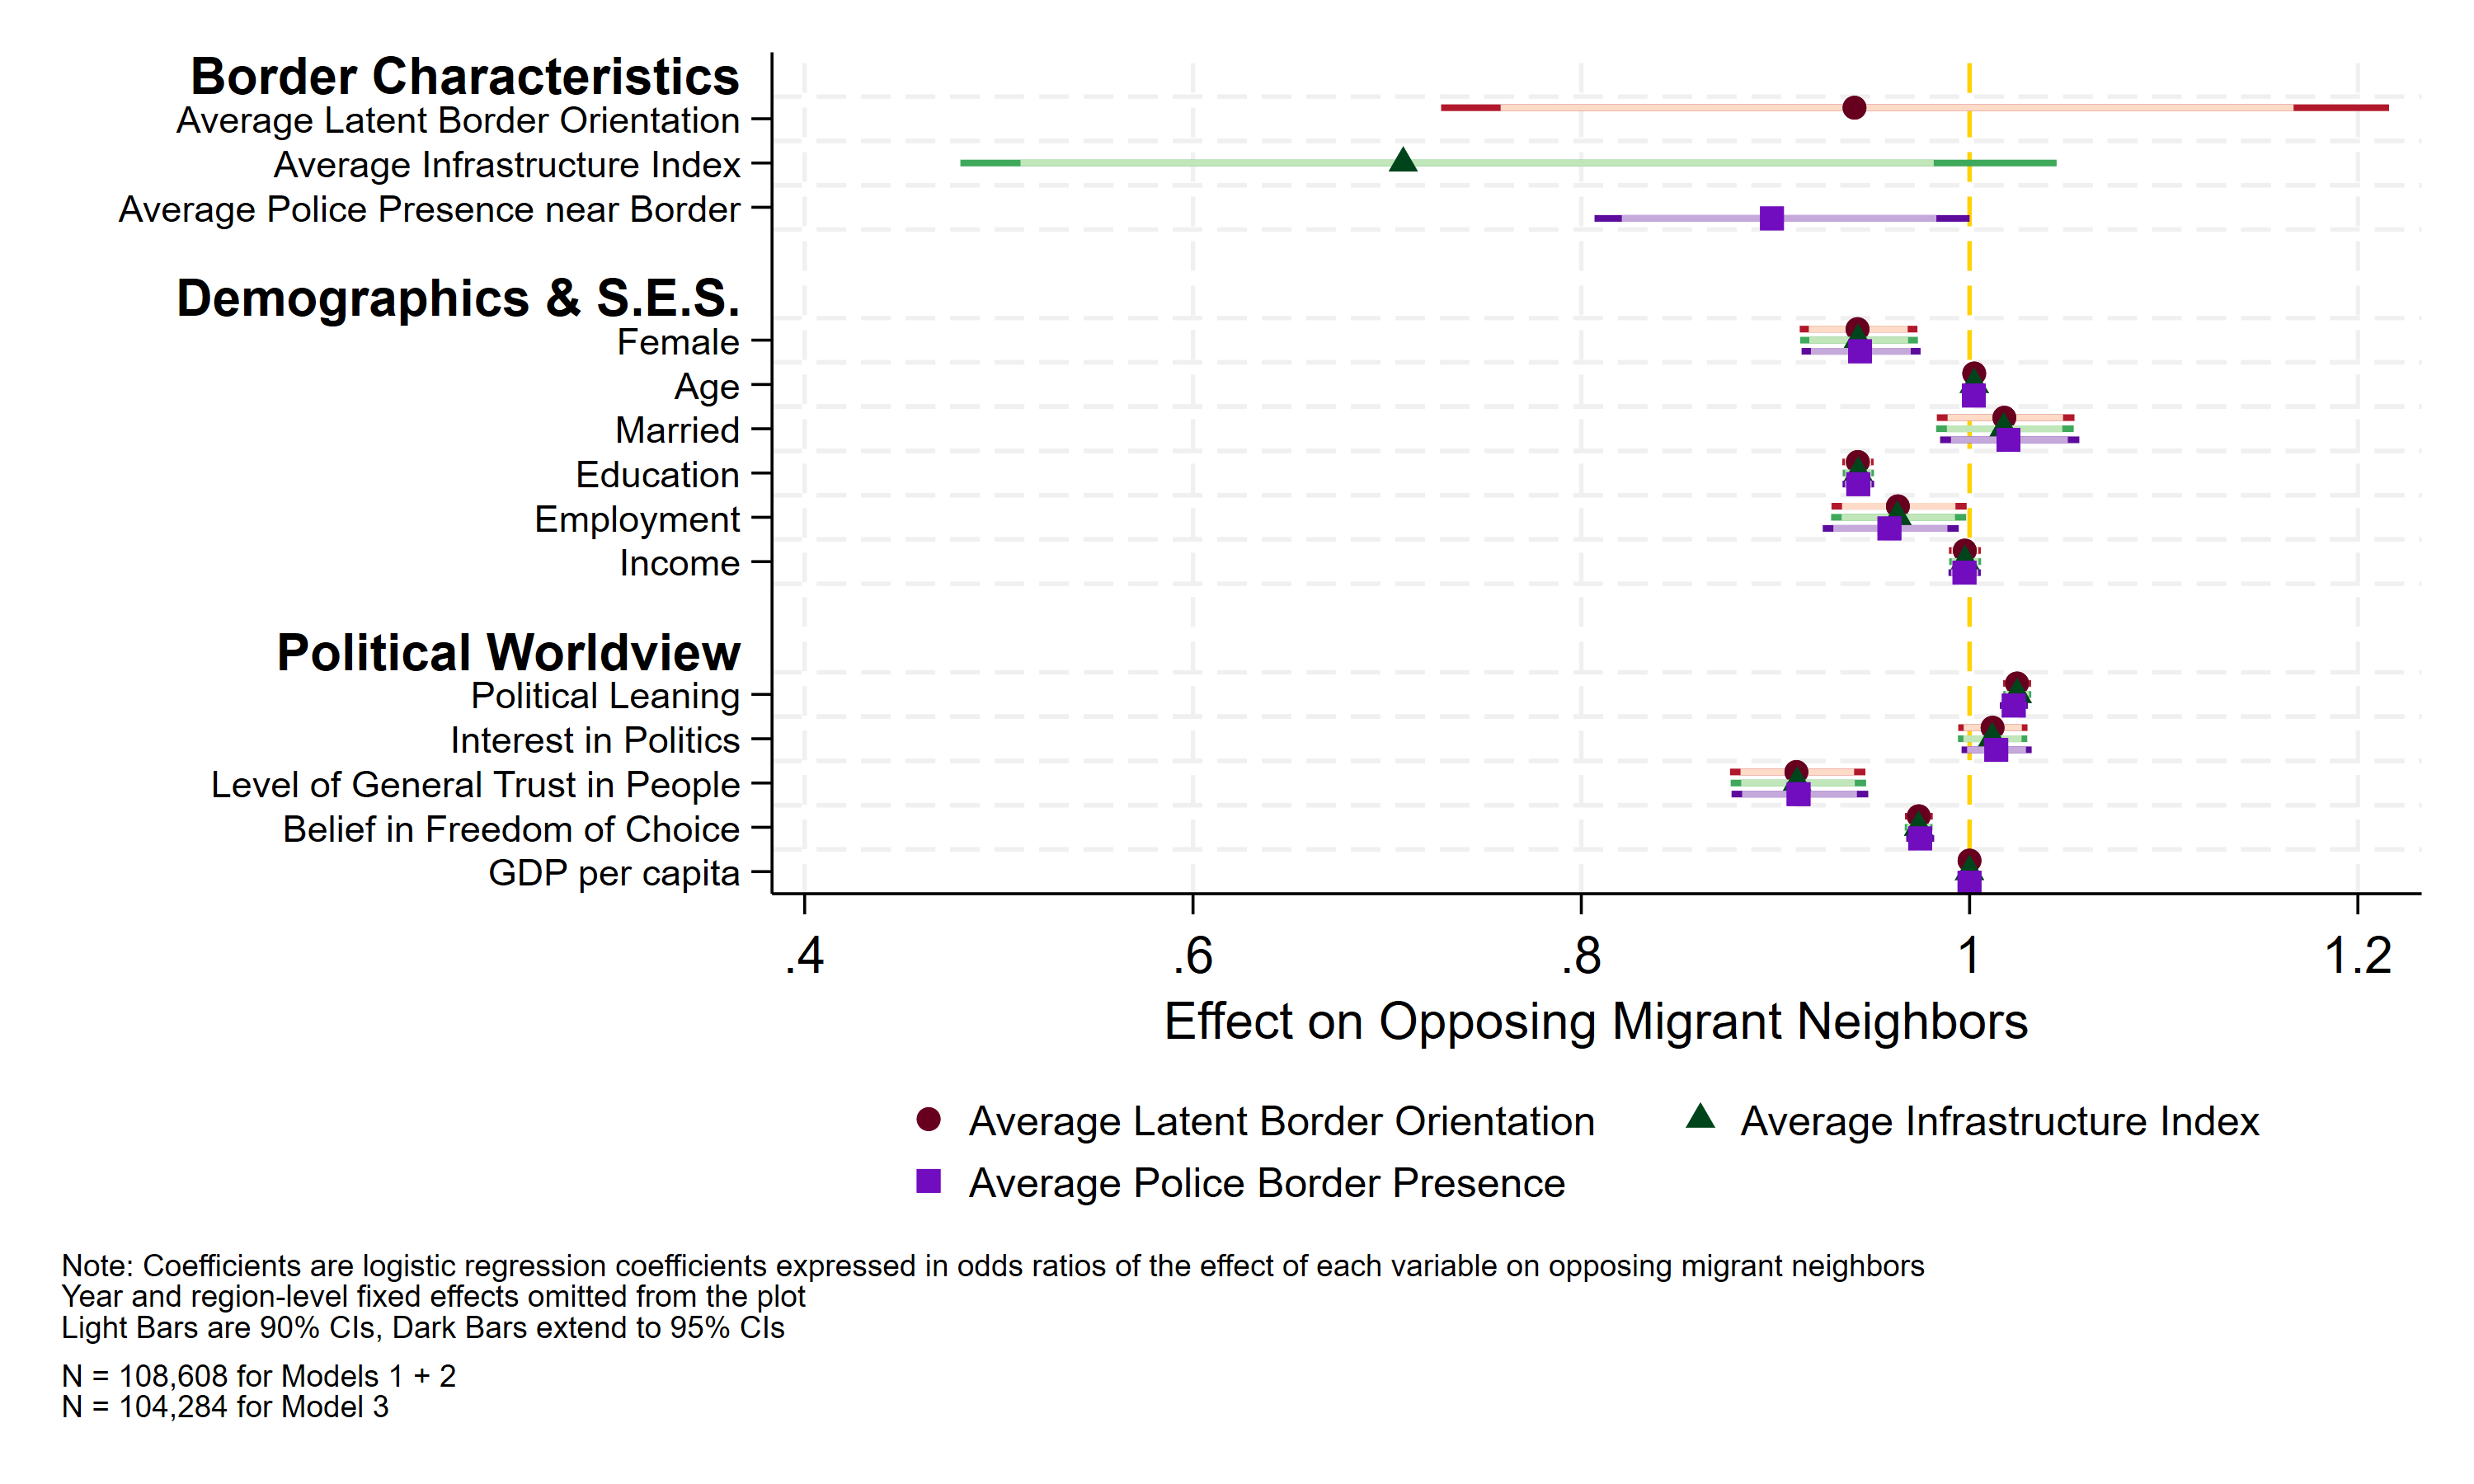
\includegraphics{figures/border_orientation_figure1.png}
\caption{Figure 1: Testing H1 - Opposing Migrant Neighbors}
\end{figure}

As Figure 1 clearly showcases, I find little statistical significance
for the border fortification variables impacting the likelihood of
opposing migrant neighbors. Interestingly, I find that a higher level of
police presence near the border results in a reduced likelihood of
opposing having migrant neighbors. As relative police presence along the
border increases, the odds of opposing migrant neighbors changes by a
factor of \textasciitilde0.90. Similarly, the other fortification
variables are also negative, albeit statistically insignificant at the
5\% level. I also find weak evidence in favor of higher levels of border
infrastructure improving attitudes towards migrants. Additionally, I
find that higher levels of trust in the public results in a lower
likelihood of opposing migrant neighbors, but higher levels of
conservatism does increase the likelihood of opposition.

Figure 2 finds generally similar results as in Figure 1 - the most
notable difference is that the police presence near the border becomes
statistically insignificant at the 5\% level. Similar to before, I find
that higher levels of conservatism result in reduced odds of supporting
more pro-immigration policies. For each one unit increase on the
left-right scale, the odds of supporting pro-immigration policy reduces
slightly. Similarly, I find that as general trust in the public
increases, the odds of supporting pro-immigration policy increases by a
factor of about 1.3 to 1.4.

Overall, I find little support for Hypothesis 1. This poses an
interesting development for the literature on immigration attitudes and
border walls as well, providing a test of a direct implication of
\citet{mutz2022}'s argument. Given previous literature on the role of
identity and perceived similarity and \citet{mutz2022}'s argument,
attitudes towards migrants should theoretically be altered. Further
investigation should be done to continue delineating the extent to which
heightened psychological distance between both sides of the border has
tangible effects on state politics. Below, I further examine my
hypotheses, running a series of models featuring interactions between my
key variables.

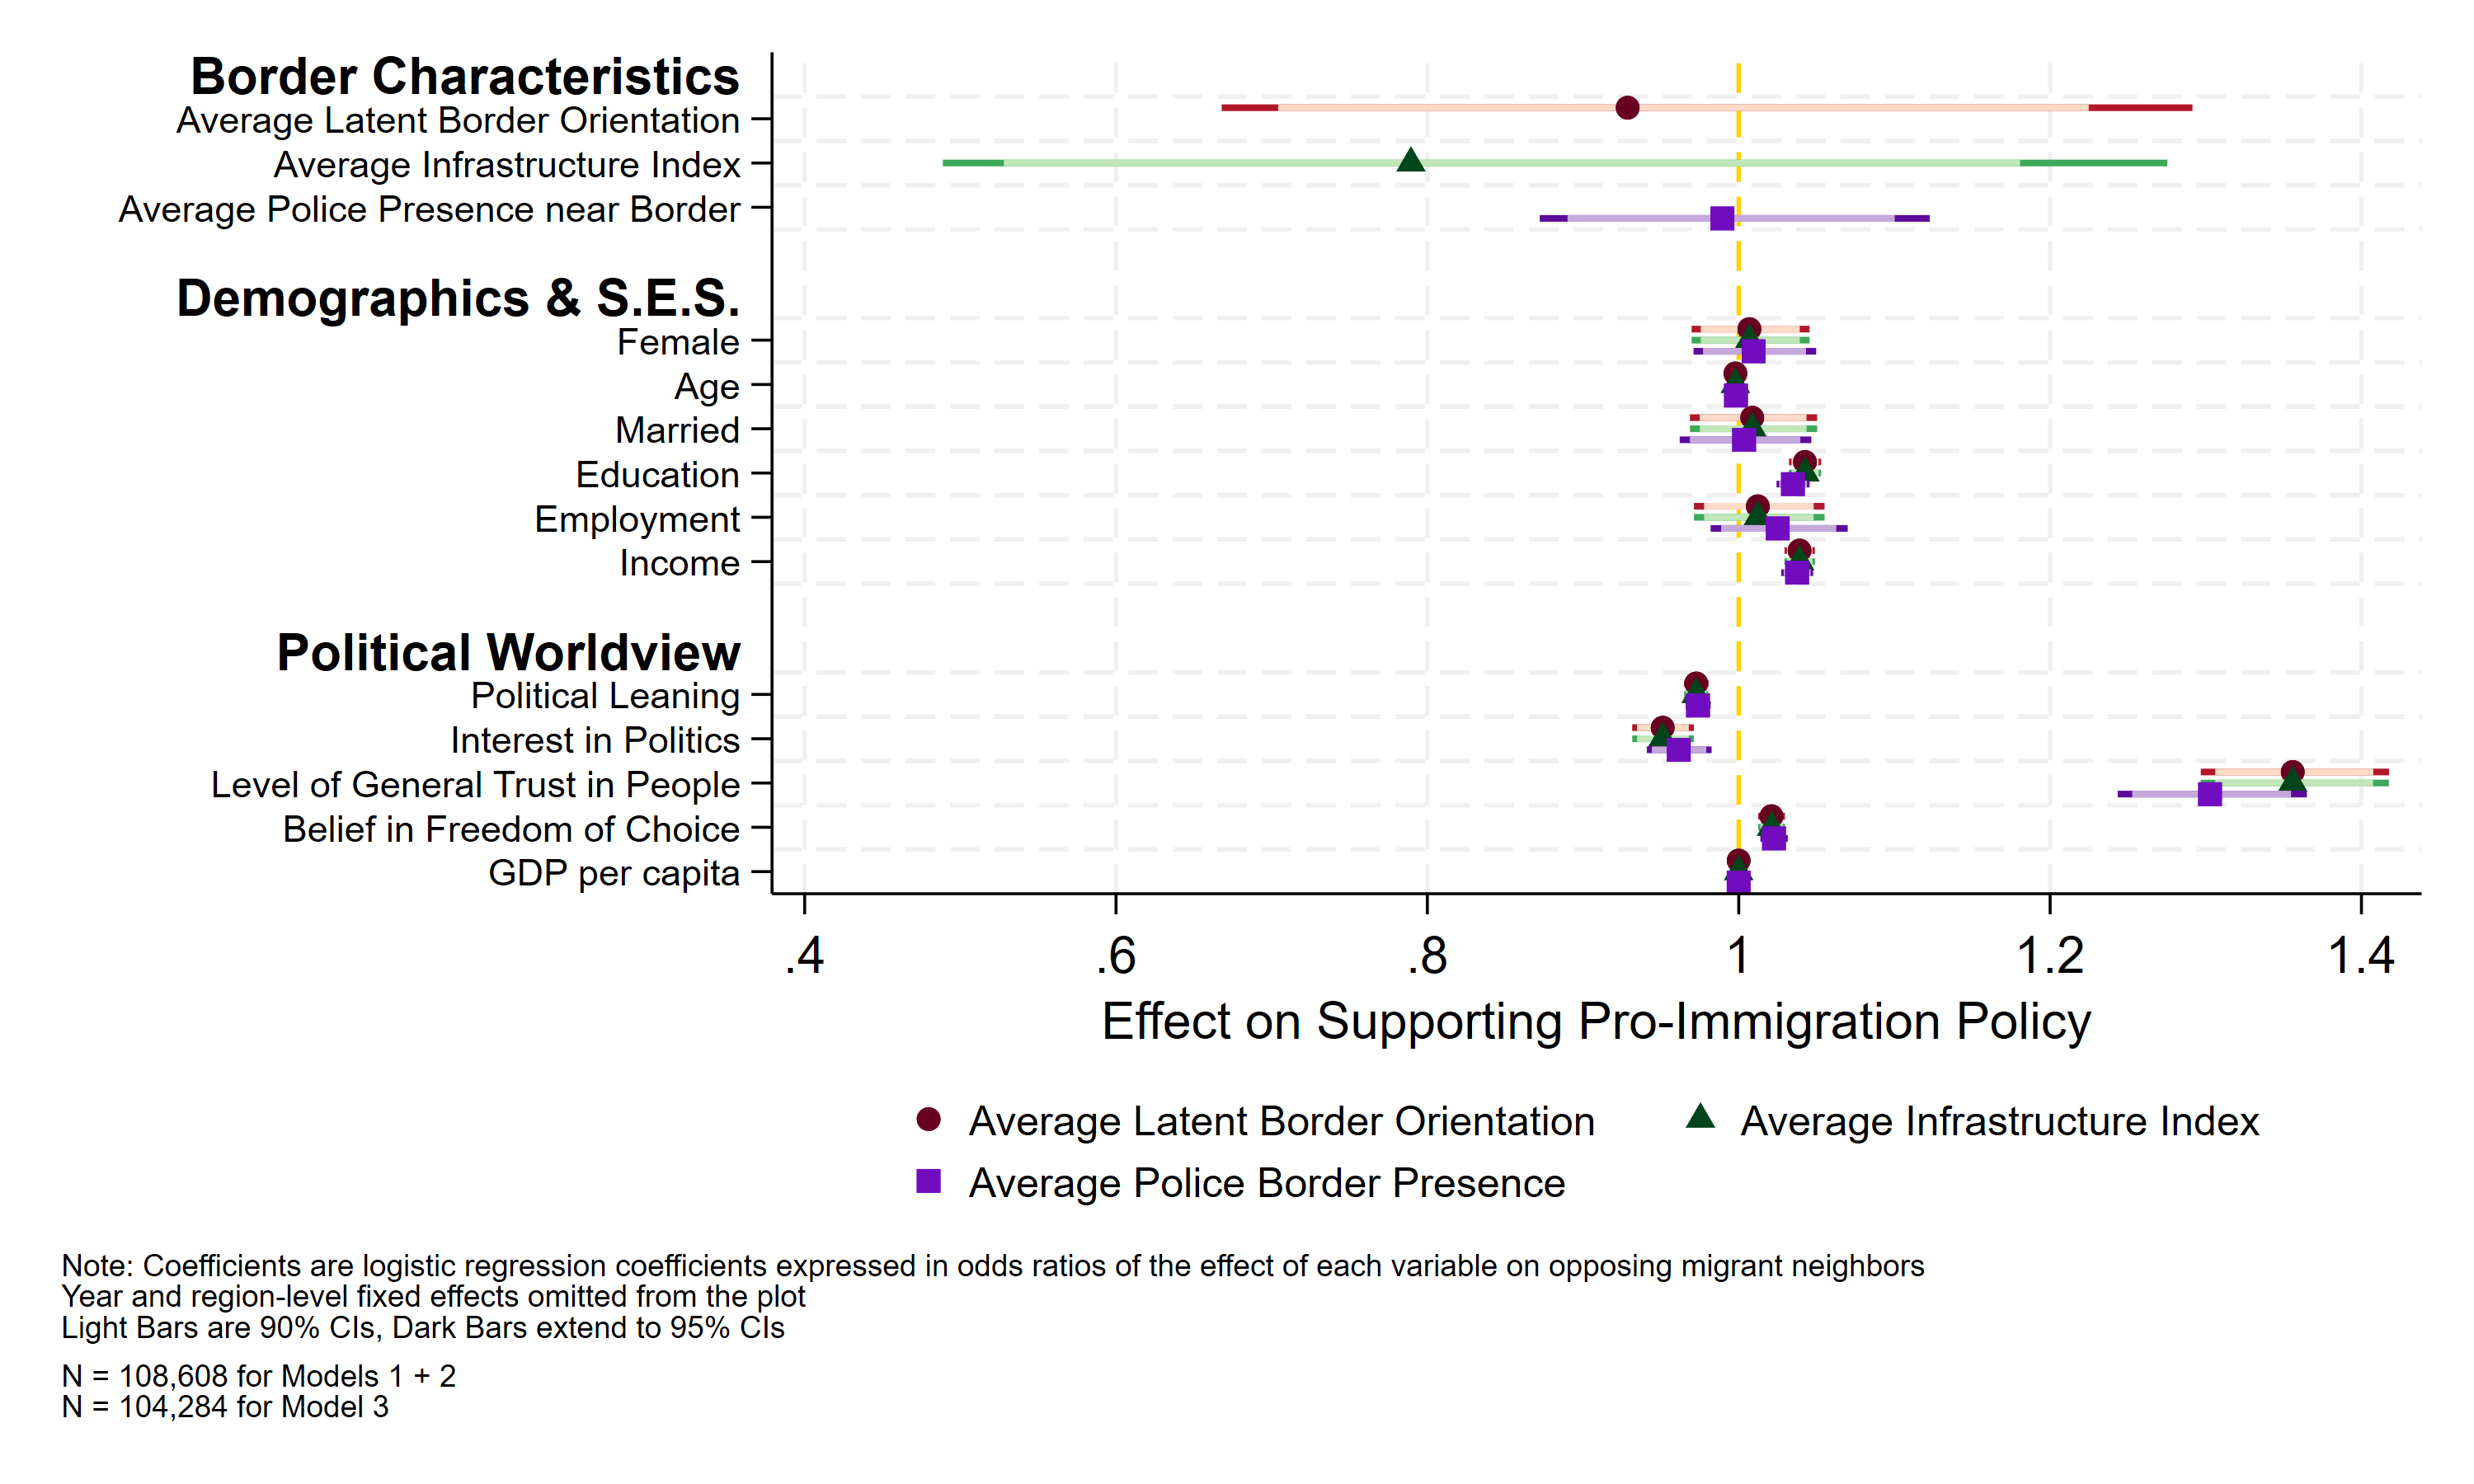
\includegraphics{figures/border_orientation_policy_figure1.png} For
Hypothesis 2, I run two models - one model where respondents' estimated
distance to the border is interacted with the border fortification
levels of the specific border that respondents are closest to, and one
where distance to the border is interacted with the state's overall
levels of border fortification. For these models, I specifically focus
on the \emph{border orientation} of the local or overall borders for the
interaction. I then estimate the marginal effects for these interactions
and depict the effect of border distance as border orientation changes,
and vice-versa. These marginal effects are depicted below in Figures 3
and 4 for the likelihood of opposing migrant neighbors and supporting
pro-immigration policy, respectively.

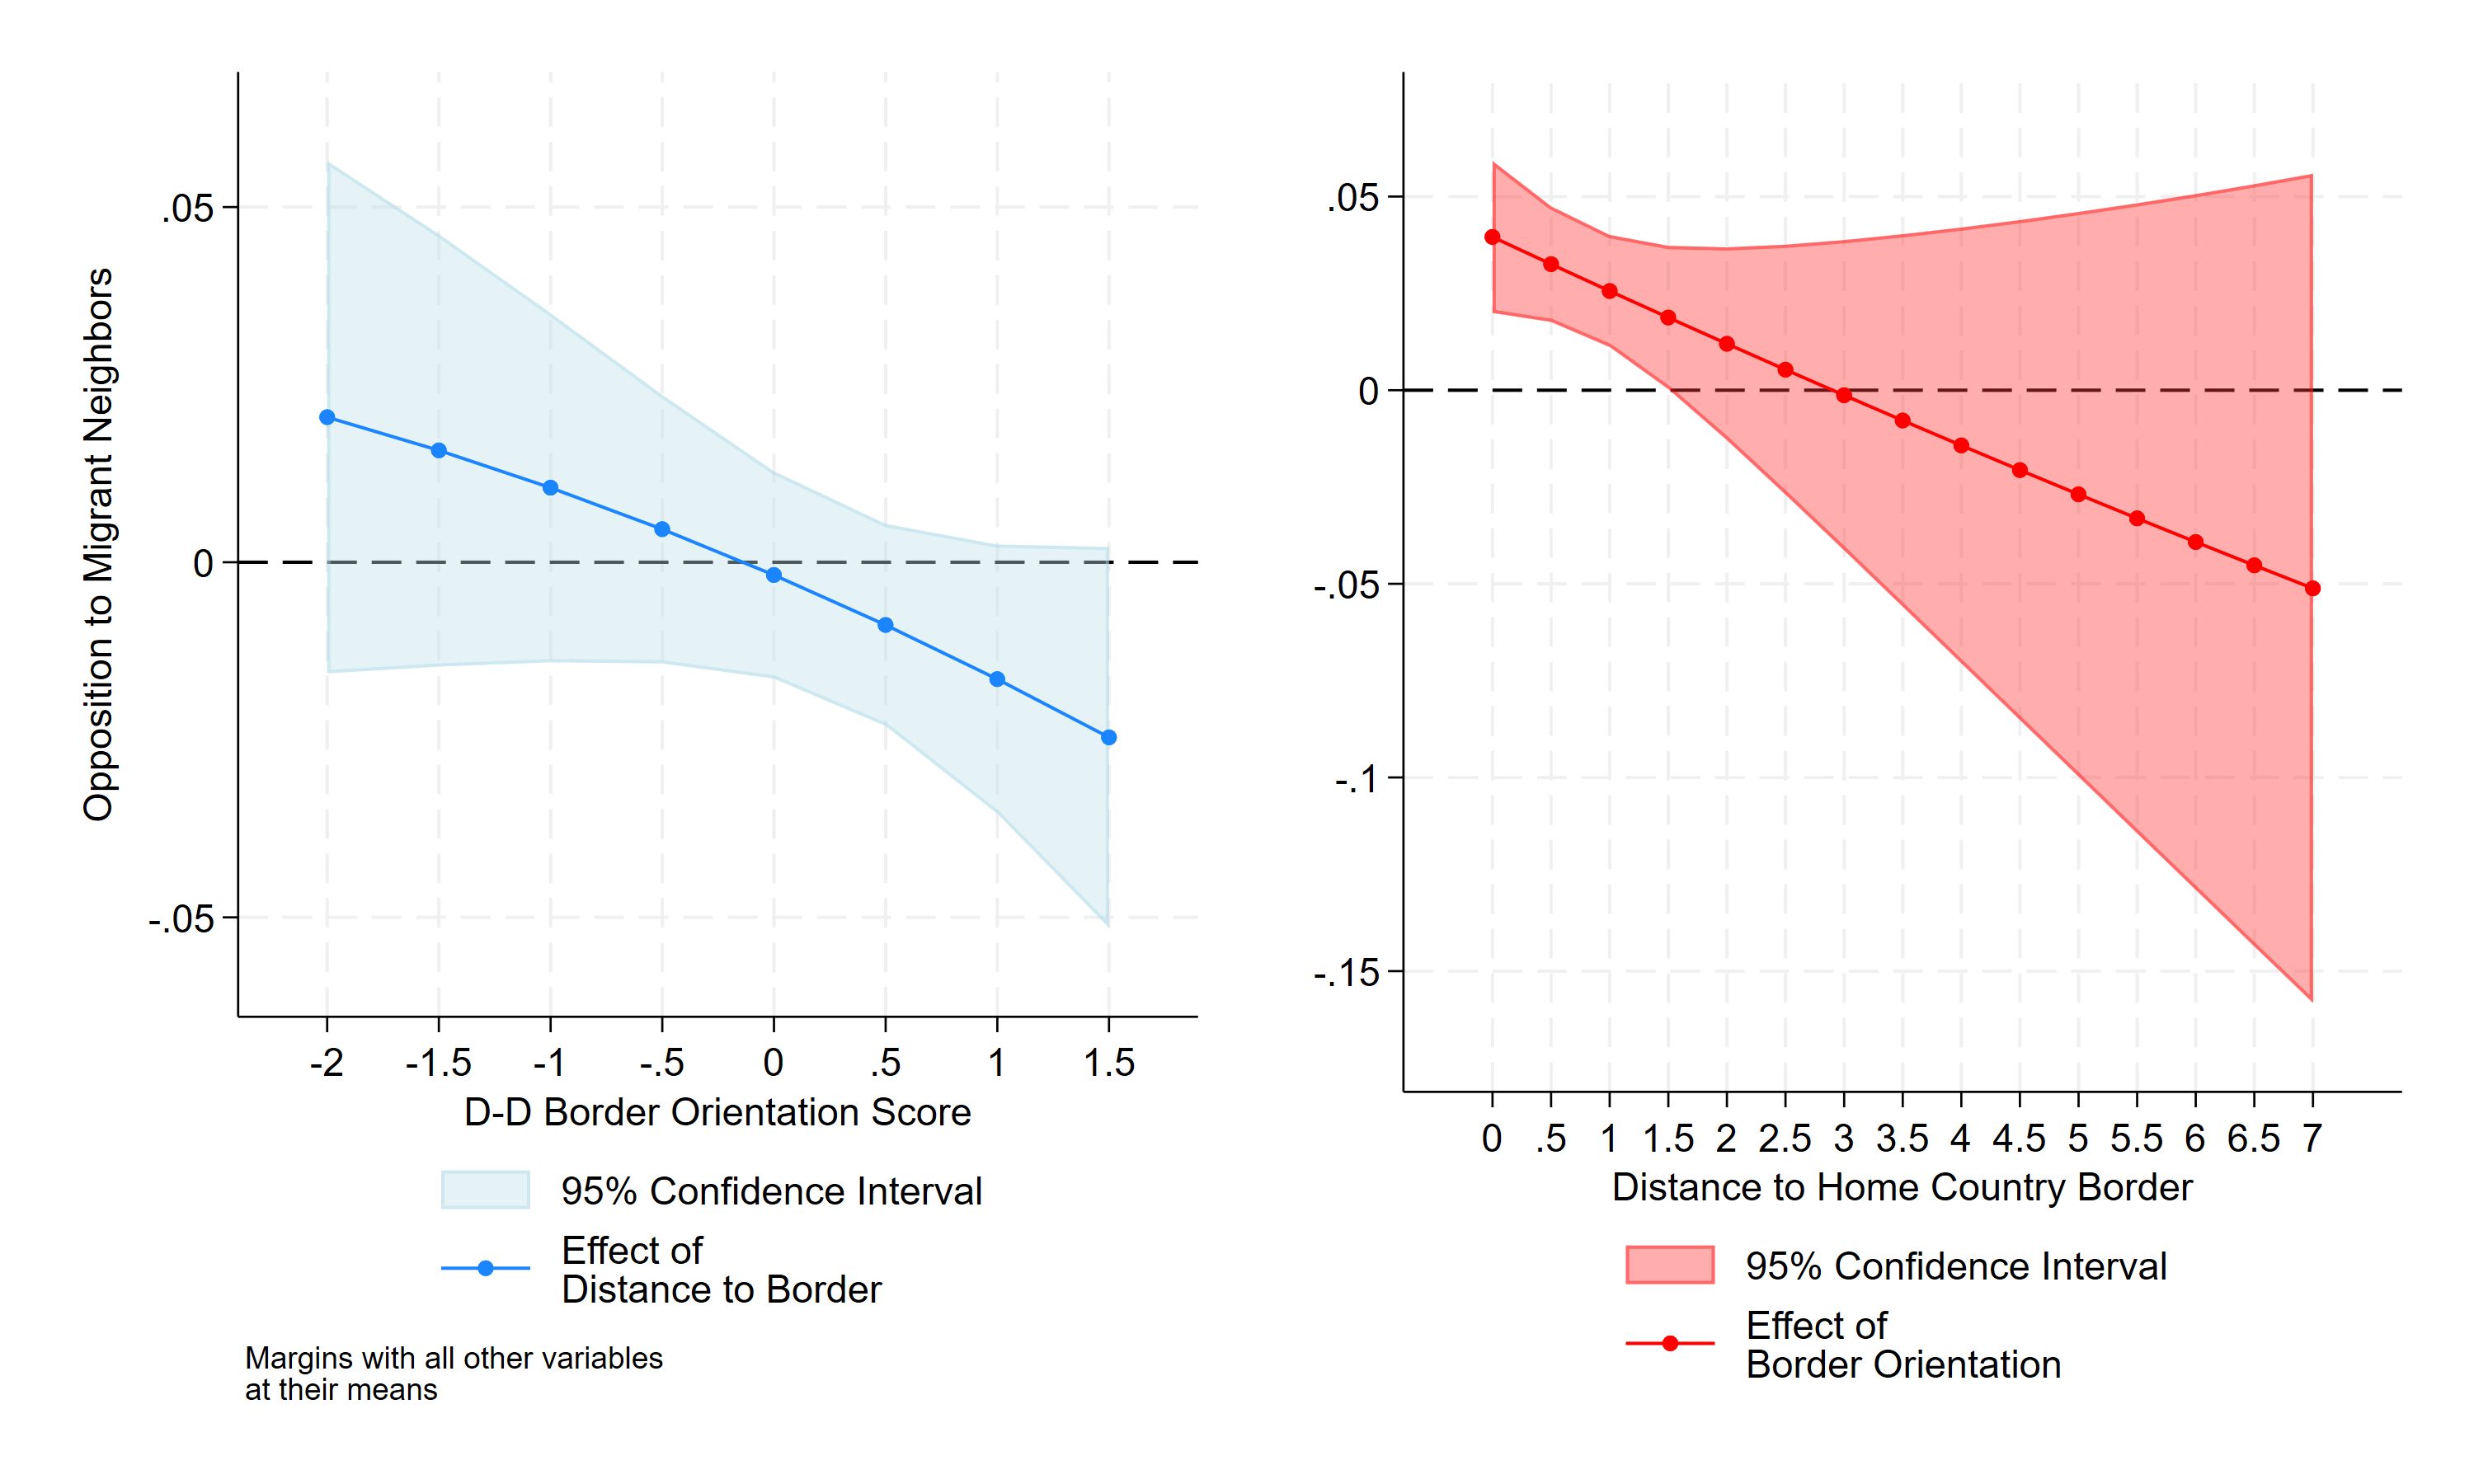
\includegraphics{figures/m4_marginal_1.png} Figure 3 shows weak evidence
in favor of Hypothesis 2a. I find that as the respondent's estimated
distance to the border increases, we see a notable decline in the effect
of border orientation. Relatedly, I find that there is little impact of
local border orientation on the effect of respondents' distance to that
border when predicting the odds of opposing having a migrant neighbor.
Figure 4 reflects similar results for Hypothesis 2a - as respondents
live further from the border, the impact of the states' overall levels
of border fortification diminishes slightly. Further, while there is
weak statistical significance, these figures reflect weak substantive
significance as well, in which increases in border distance change the
coefficient for border distance by only a mere fraction before reaching
statistical insignificance. Ultimately, I find little support for the
interactive effects of local border fortifications and border distance
on attitudes related to migrants themselves.

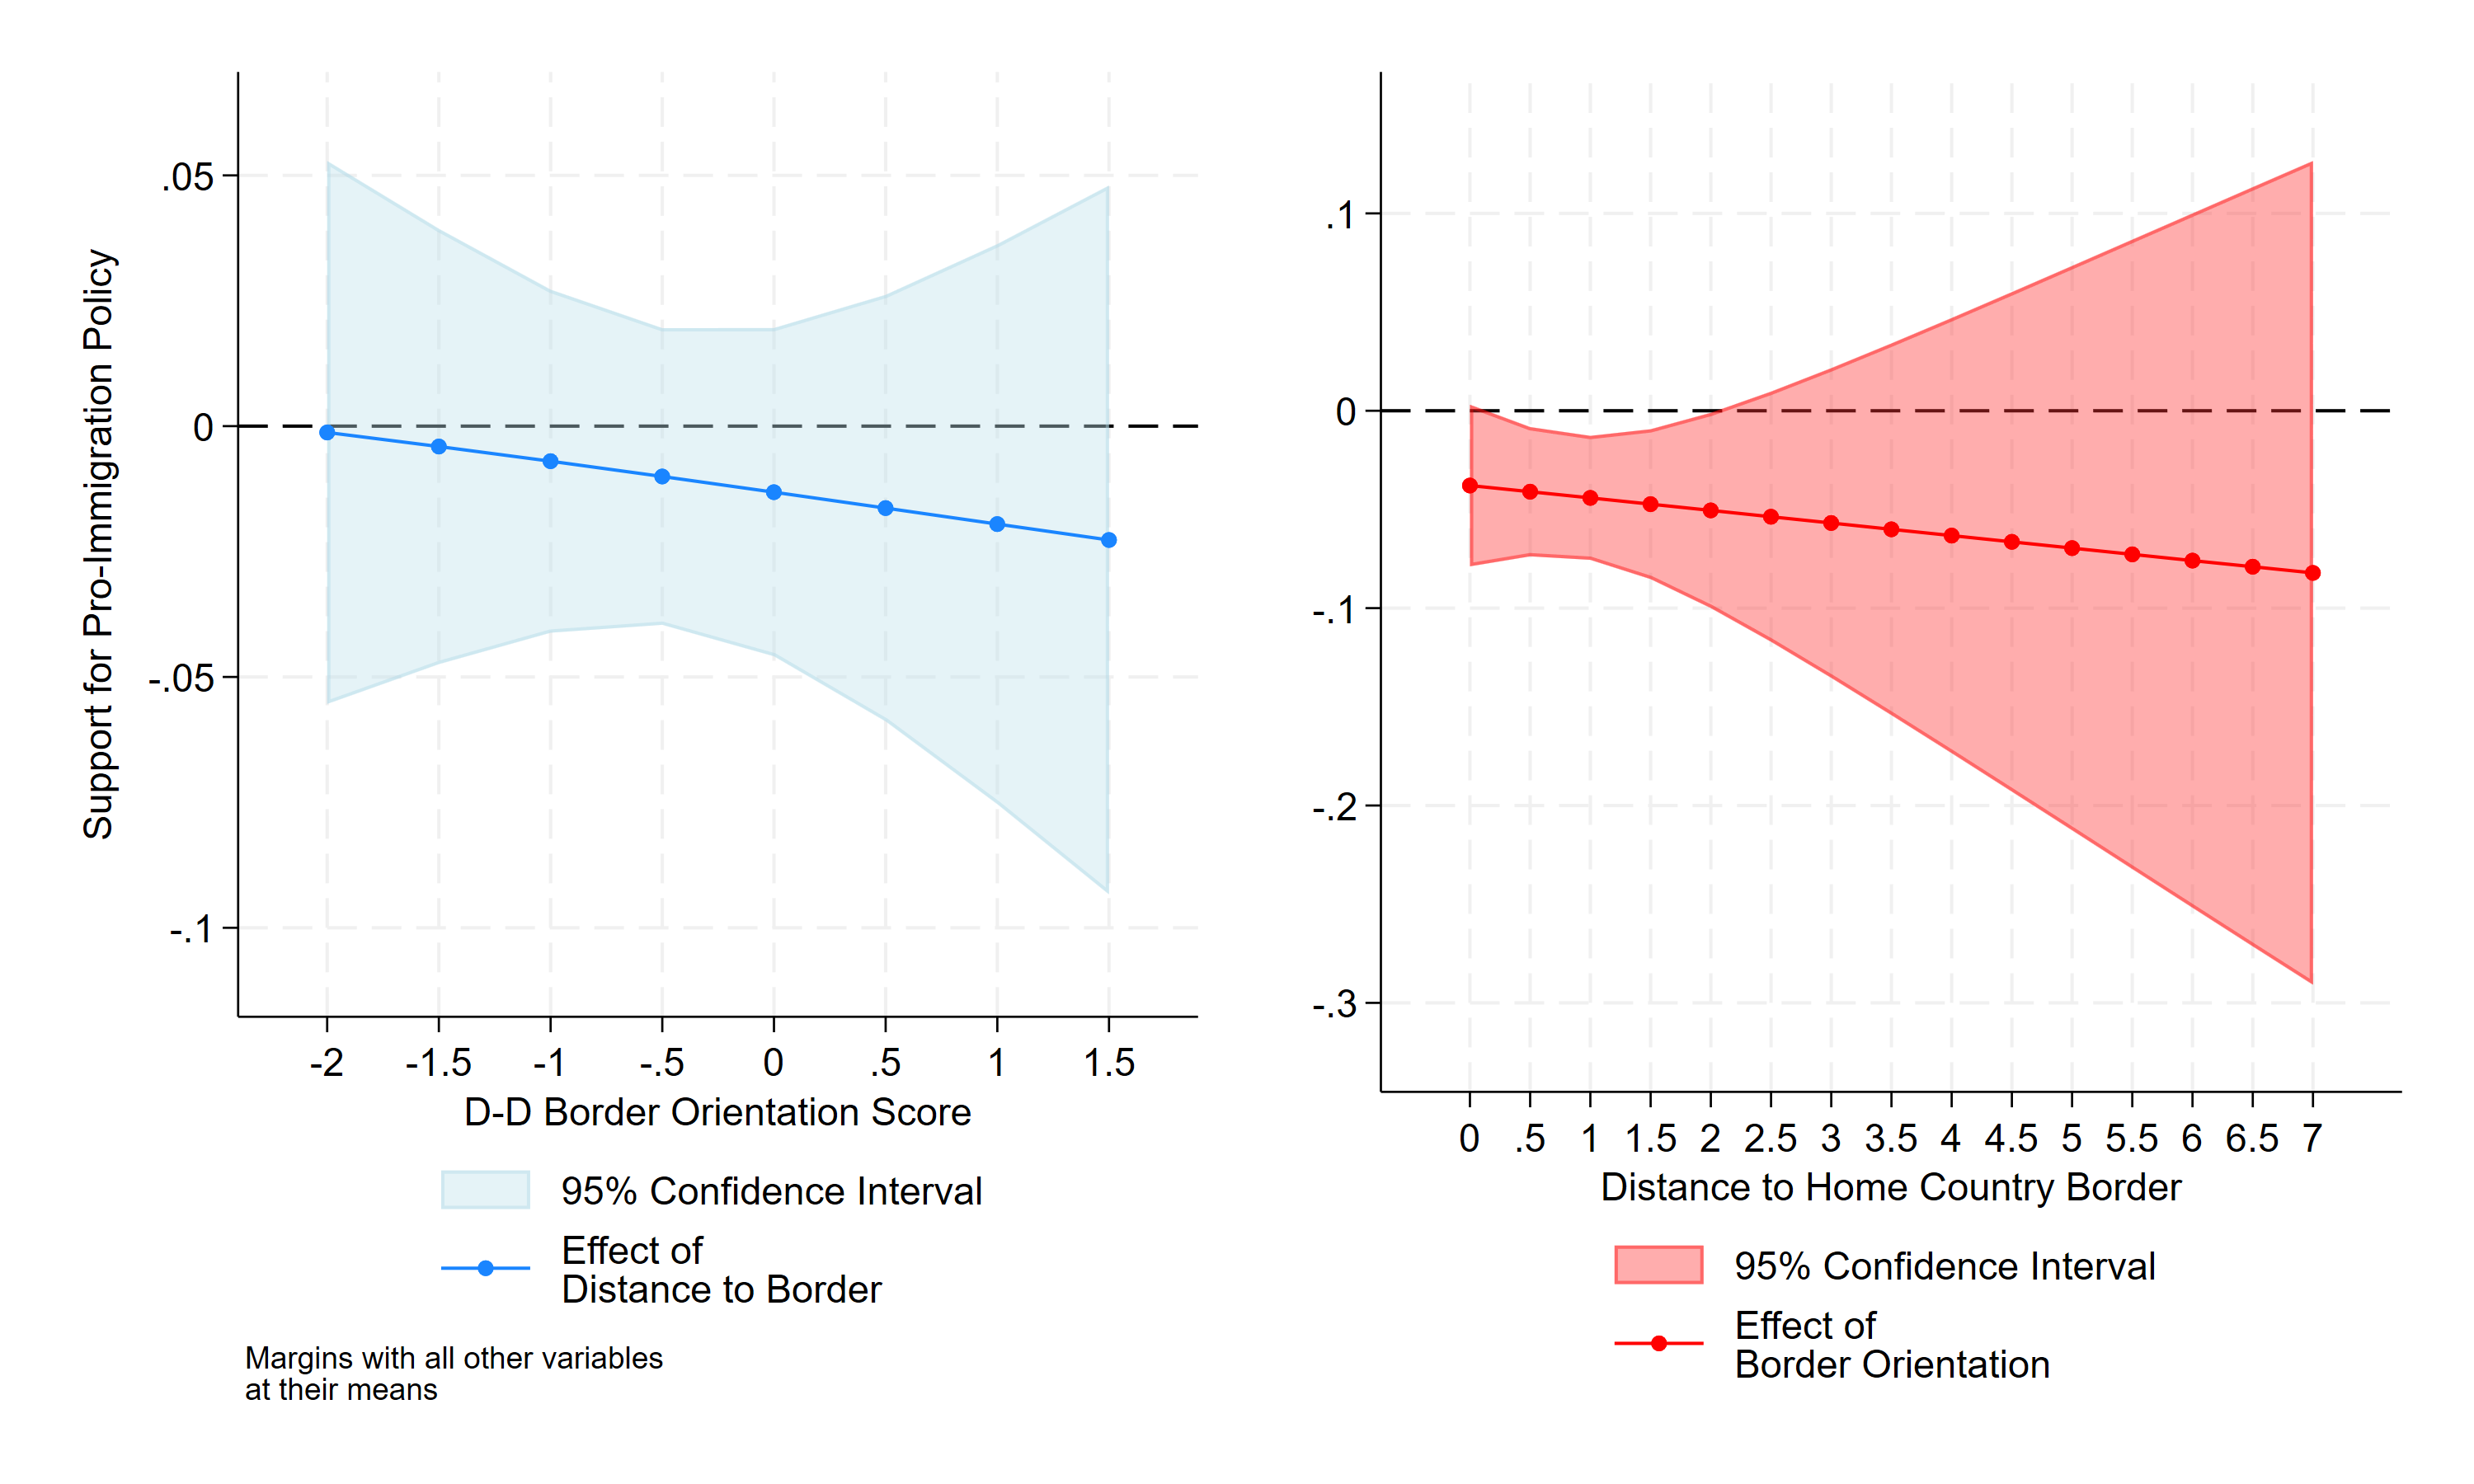
\includegraphics{figures/m4_policy_marginal_1.png} Investigations into
how distance to the border impacts the effect of border fortifications
on respondent attitudes shows similarly poor findings. In Figure 5, I
find that as distance increases, there is a slight positive uptick on
the effect of overall border fortifications on opposing migrant
neighbors, although the results and their corresponding confidence
interval are largely flat, indicating a generally consistent effect for
border fortifications as distance increases. Figure 6 reflects little
evidence for the interaction's impact on support for pro-immigration
policy as well. While the trend is clearly positive, the results are
ultimately within the confidence interval and cross the 0 mark. While
the effect of border orientation statewide becomes more positive as
distance increases, indicating that more controlling border orientations
result in more support for migrants the further they live from said
border, the results are ultimately statistically insignificant. While
this provides some suggestive evidence that border orientation may
result in almost a thermostatic backlash for those who do not actually
live near said policies, providing a potential path for exploration in
the future, the results here do not showcase significance for such a
claim.

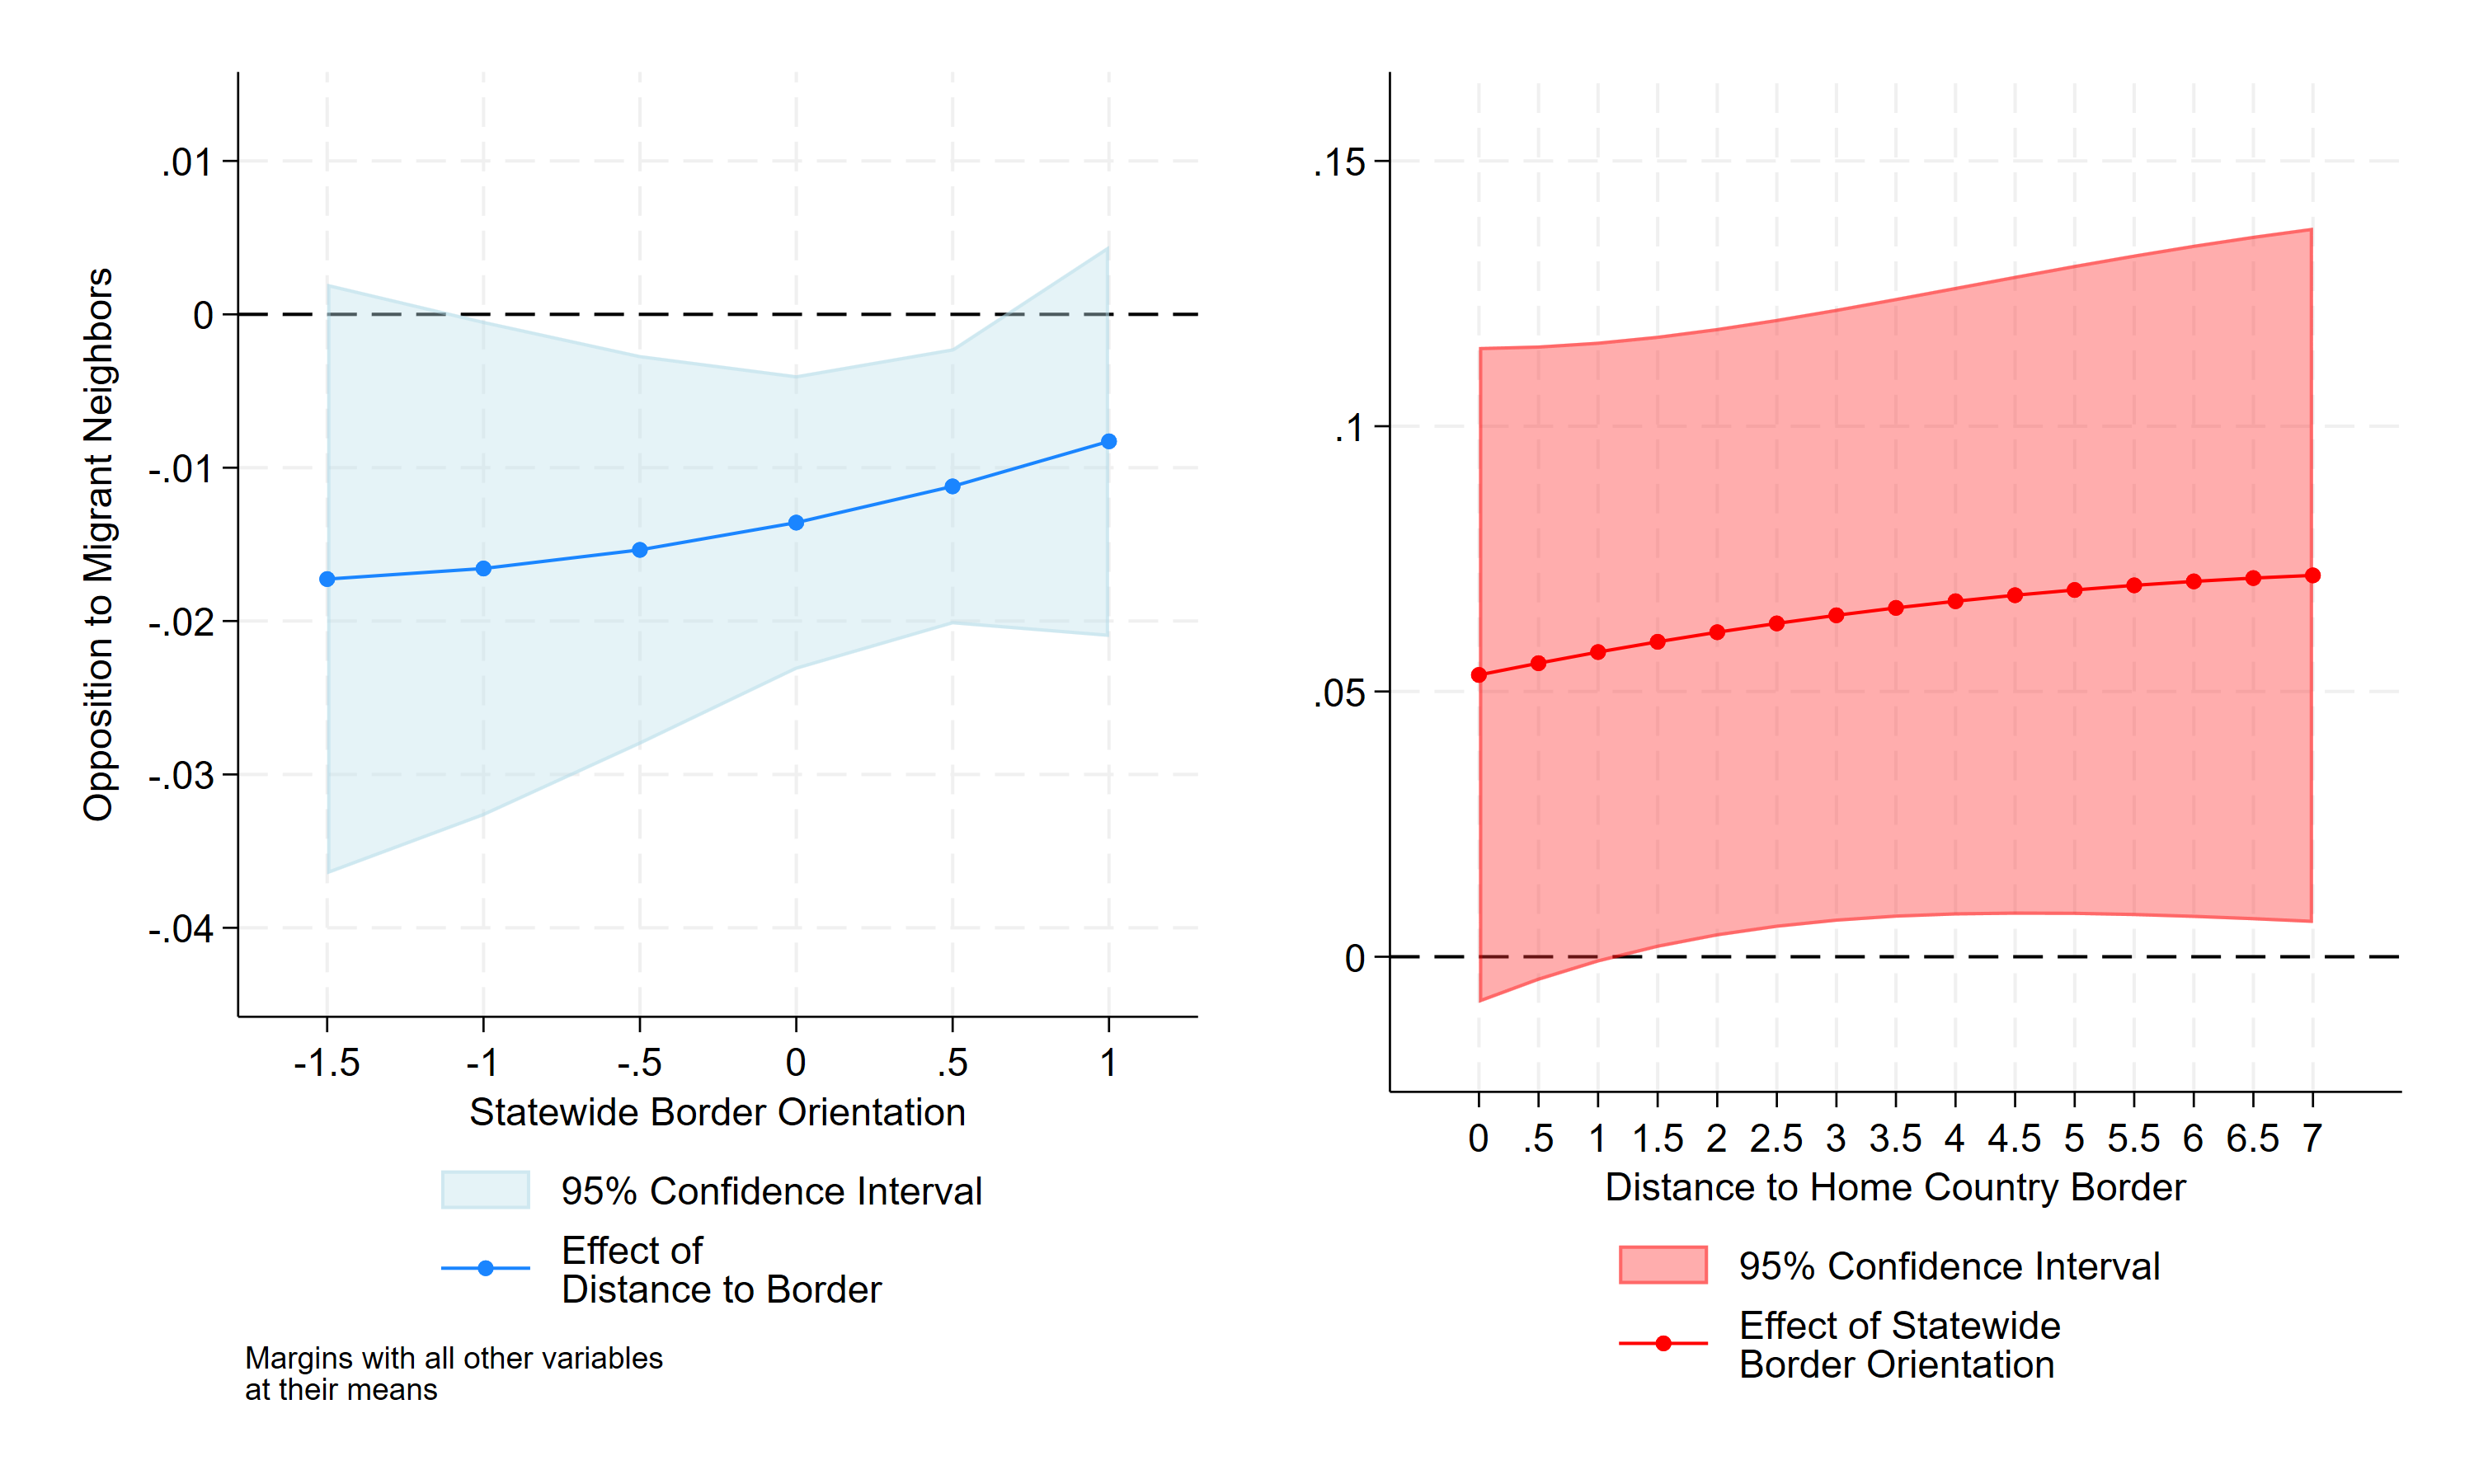
\includegraphics{figures/m4a_marginal_1.png} However, Figure 6 finds a
clear positive trend for opposition increasing the impact of border
distance - as the overall border orientation of the state becomes more
controlling, distance to the border shifts from having a negative impact
on the likelihood of support for pro-immigration policy to a positive
one. This indicates that as respondents live in increasingly controlling
(at least on the border) states, the further away they are from said
border, the more likely they are to support pro-immigration policy. This
again provides some indication that border orientation may result in a
thermostatic backlash for respondents who live far away from the border,
but a policy-affirming feedback loop from those who live close to said
controlling borders. Ultimately, I find little evidence in favor of
Hypothesis 2b, but I find a potential direction for future research as
well.

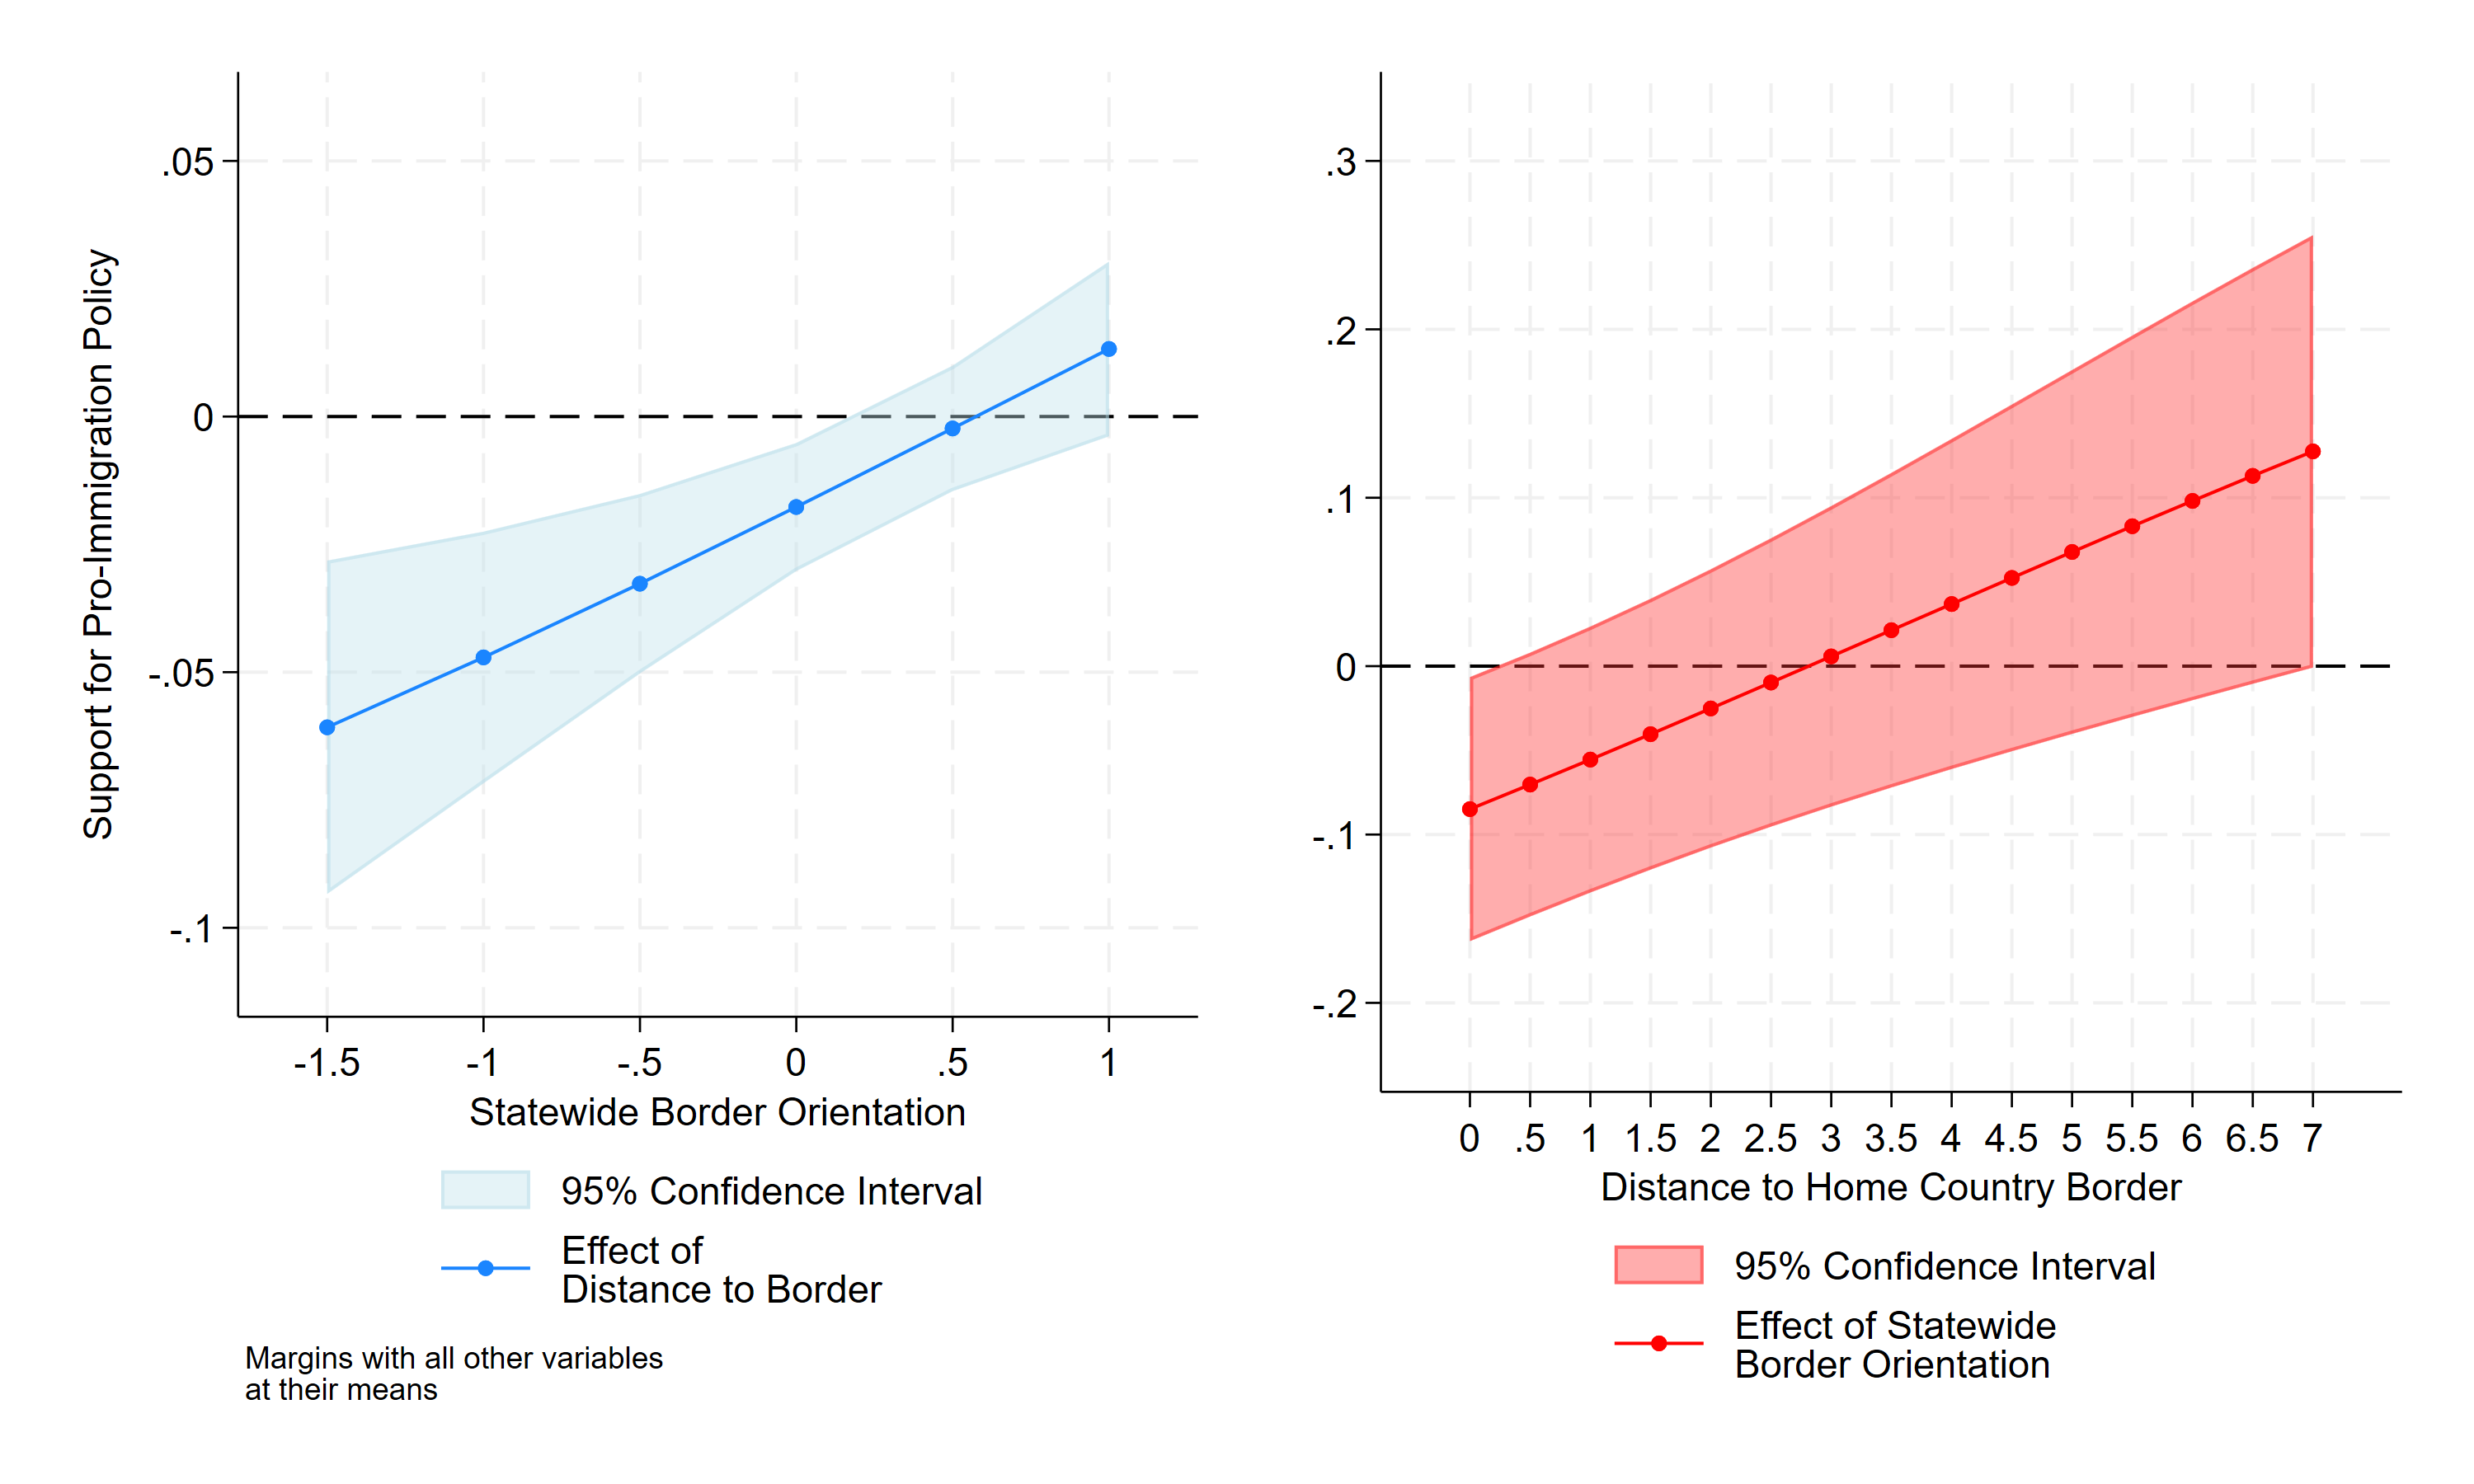
\includegraphics{figures/m4a_policy_marginal_1.png} When investigating
Hypothesis 3, that as border distance increases, the effect of increased
conservatism will become more negative towards migrants and
pro-immigration policy, I find mixed results. First, in Figure 7, when
looking at the interaction's impact on opposing migrant neighbors, I
find that as distance to the border increases, an increase in the scale
towards conservatism results in a reduced likelihood of opposing
migrants, although this quickly loses significance. Interestingly,
however, I find that as respondents become more conservative in their
self-identification, distance to the border has a stronger negative
impact on their likelihood of opposing migrants. This suggests, contrary
to the hypothesis, that distance to the border may be more relevant for
conservative-leaning individuals in reducing their opposition to migrant
neighbors, even if the role of conservatism itself on opposition is
unchanged.

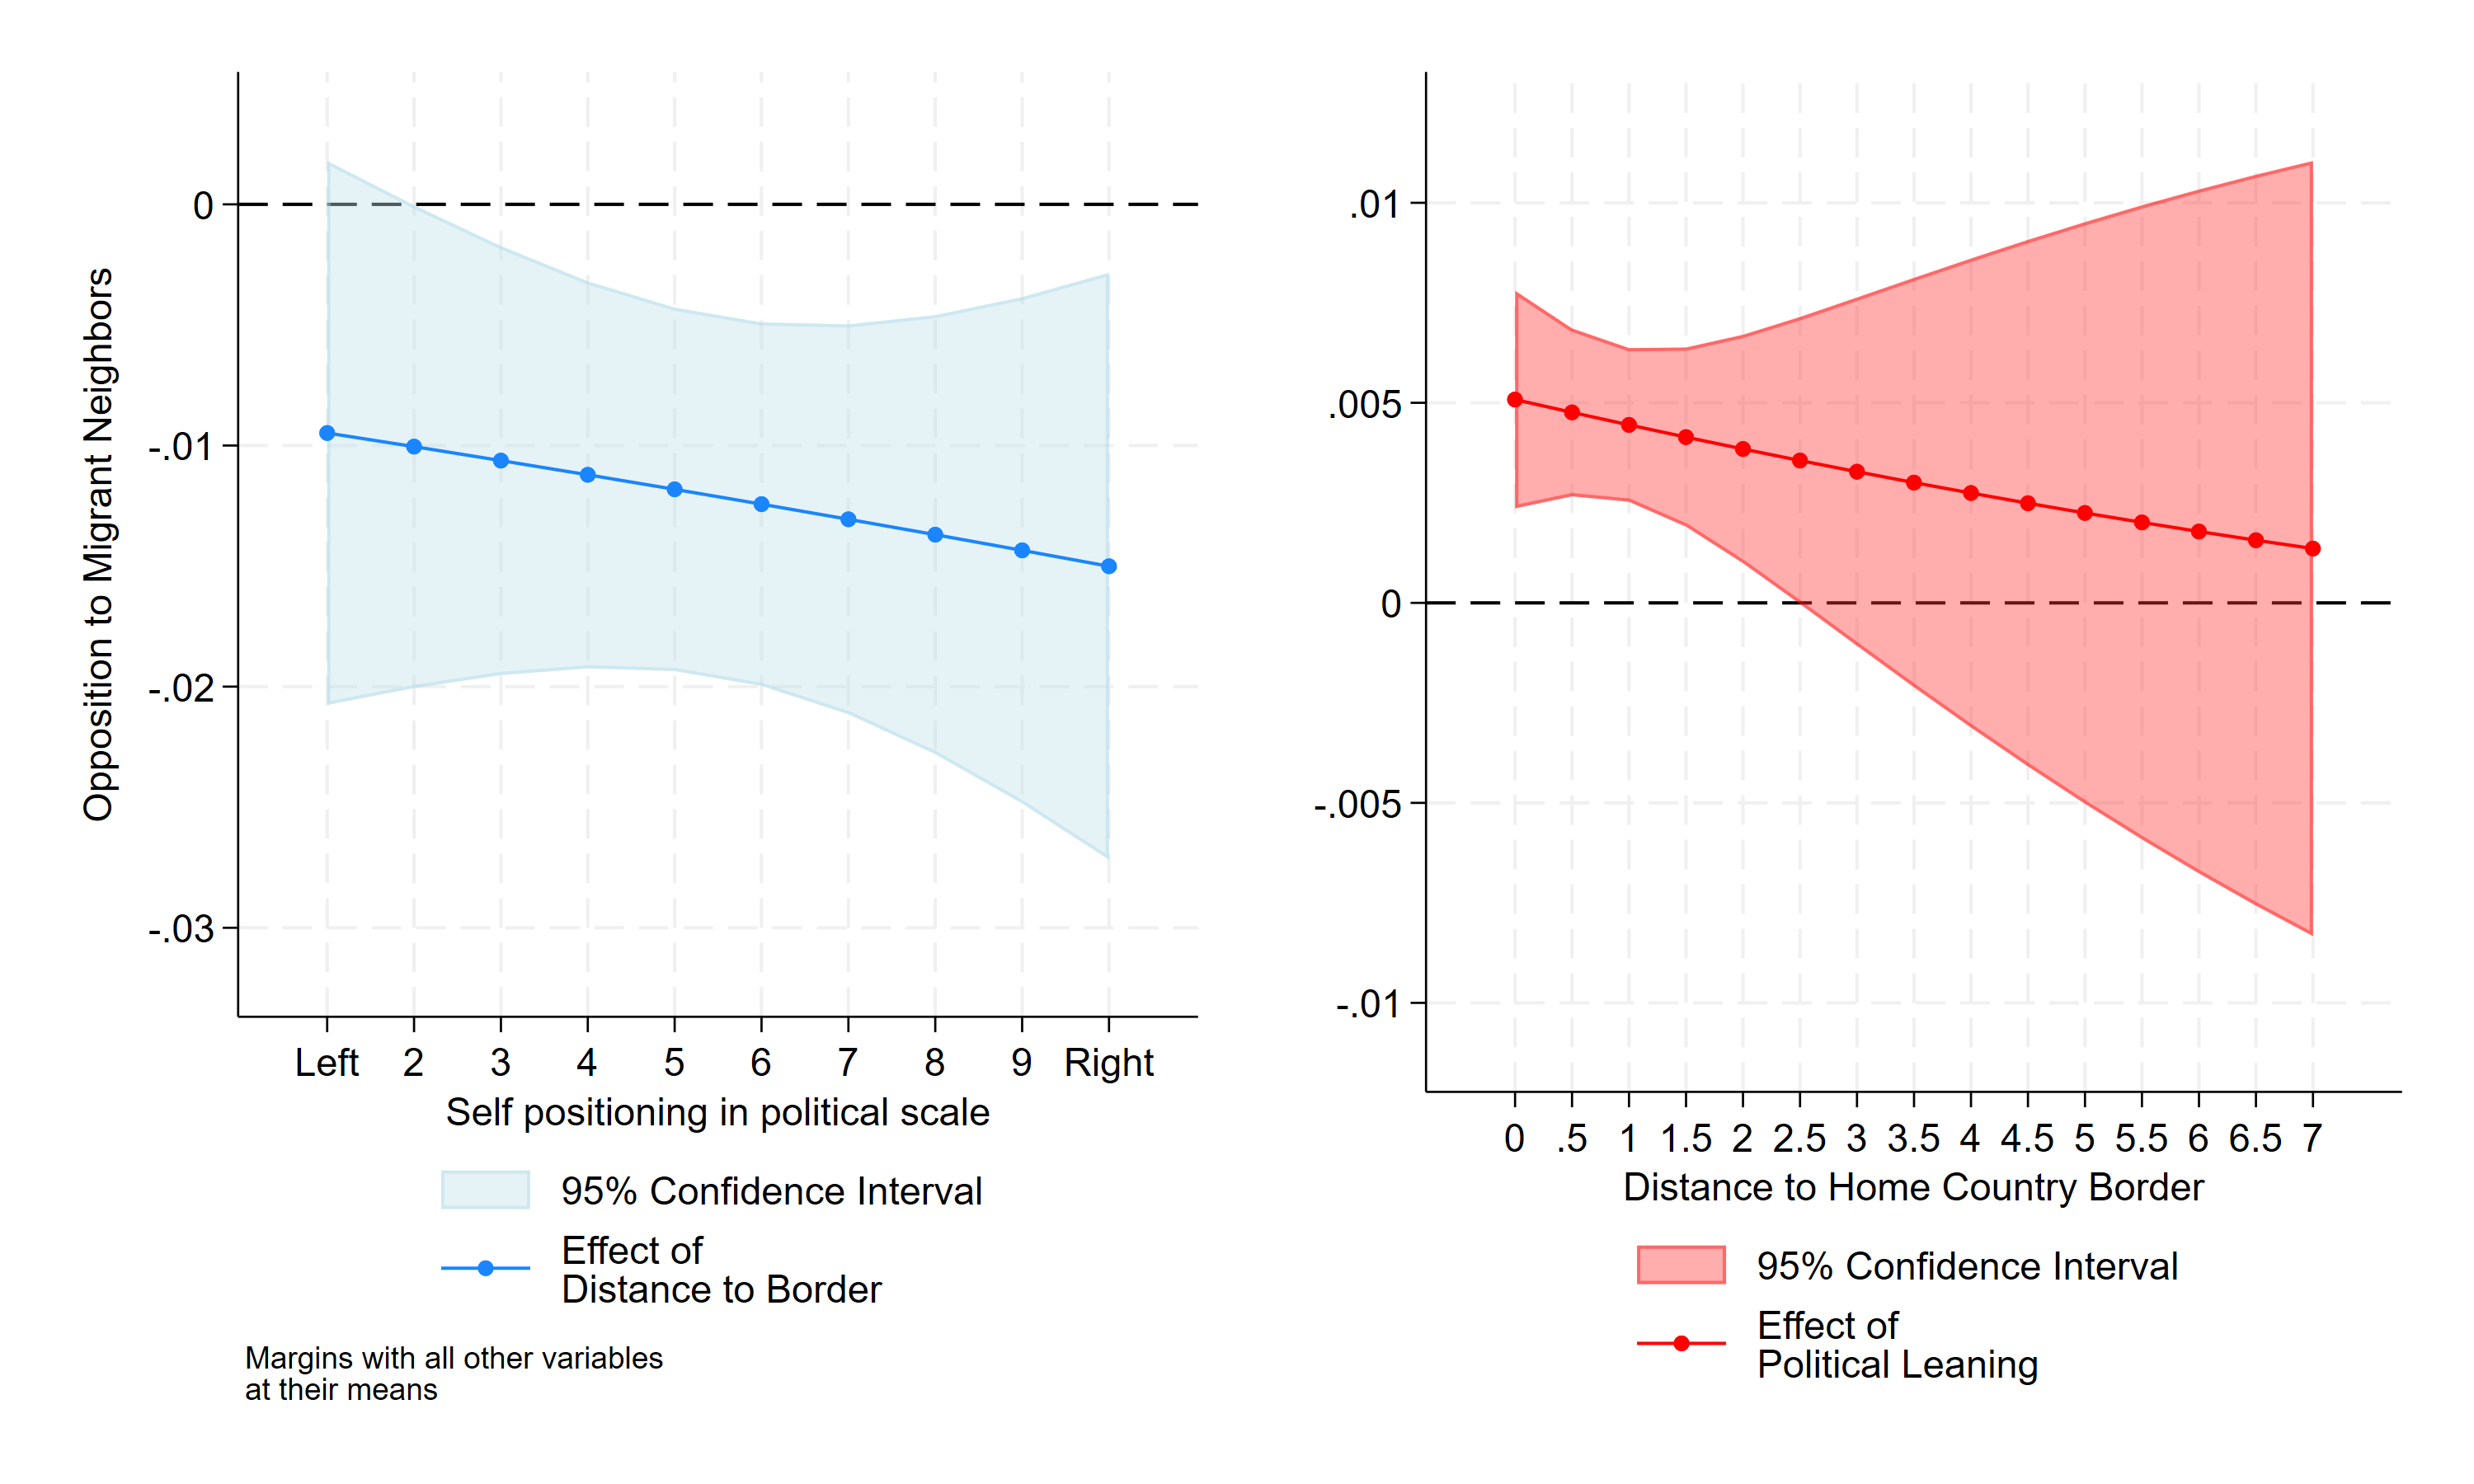
\includegraphics{figures/m5_marginal_1.png} Figure 8, however, shows
clear support for Hypothesis 3. As distance to the border increases, the
effect of respondents' self-identification becomes increasingly
negative, indicating a lower likelihood of supporting pro-immigrant
policy. In conjunction with Figure 7, this may indicate that the role of
distance and intergroup contact could impact conservatives positively
when it comes to policy opinions, even if their opinions on migrants
themselves remain negative despite such contact. However, I find no
significance for the impact of distance to the border on support for
pro-immigration policy changing as respondents' ideology shifts.
Ultimately, I find mixed evidence for Hypothesis 3 - as respondents live
further from the border, the impact of conservatism on the likelihood of
opposing migrants decreases slightly, but their likelihood of supporting
pro-immigration policy declines as well. This mixed finding suggests
further research may prove fruitful to disentangle the role of
intergroup contact on policy attitudes from its role towards potential
stigmatization or prejudice.

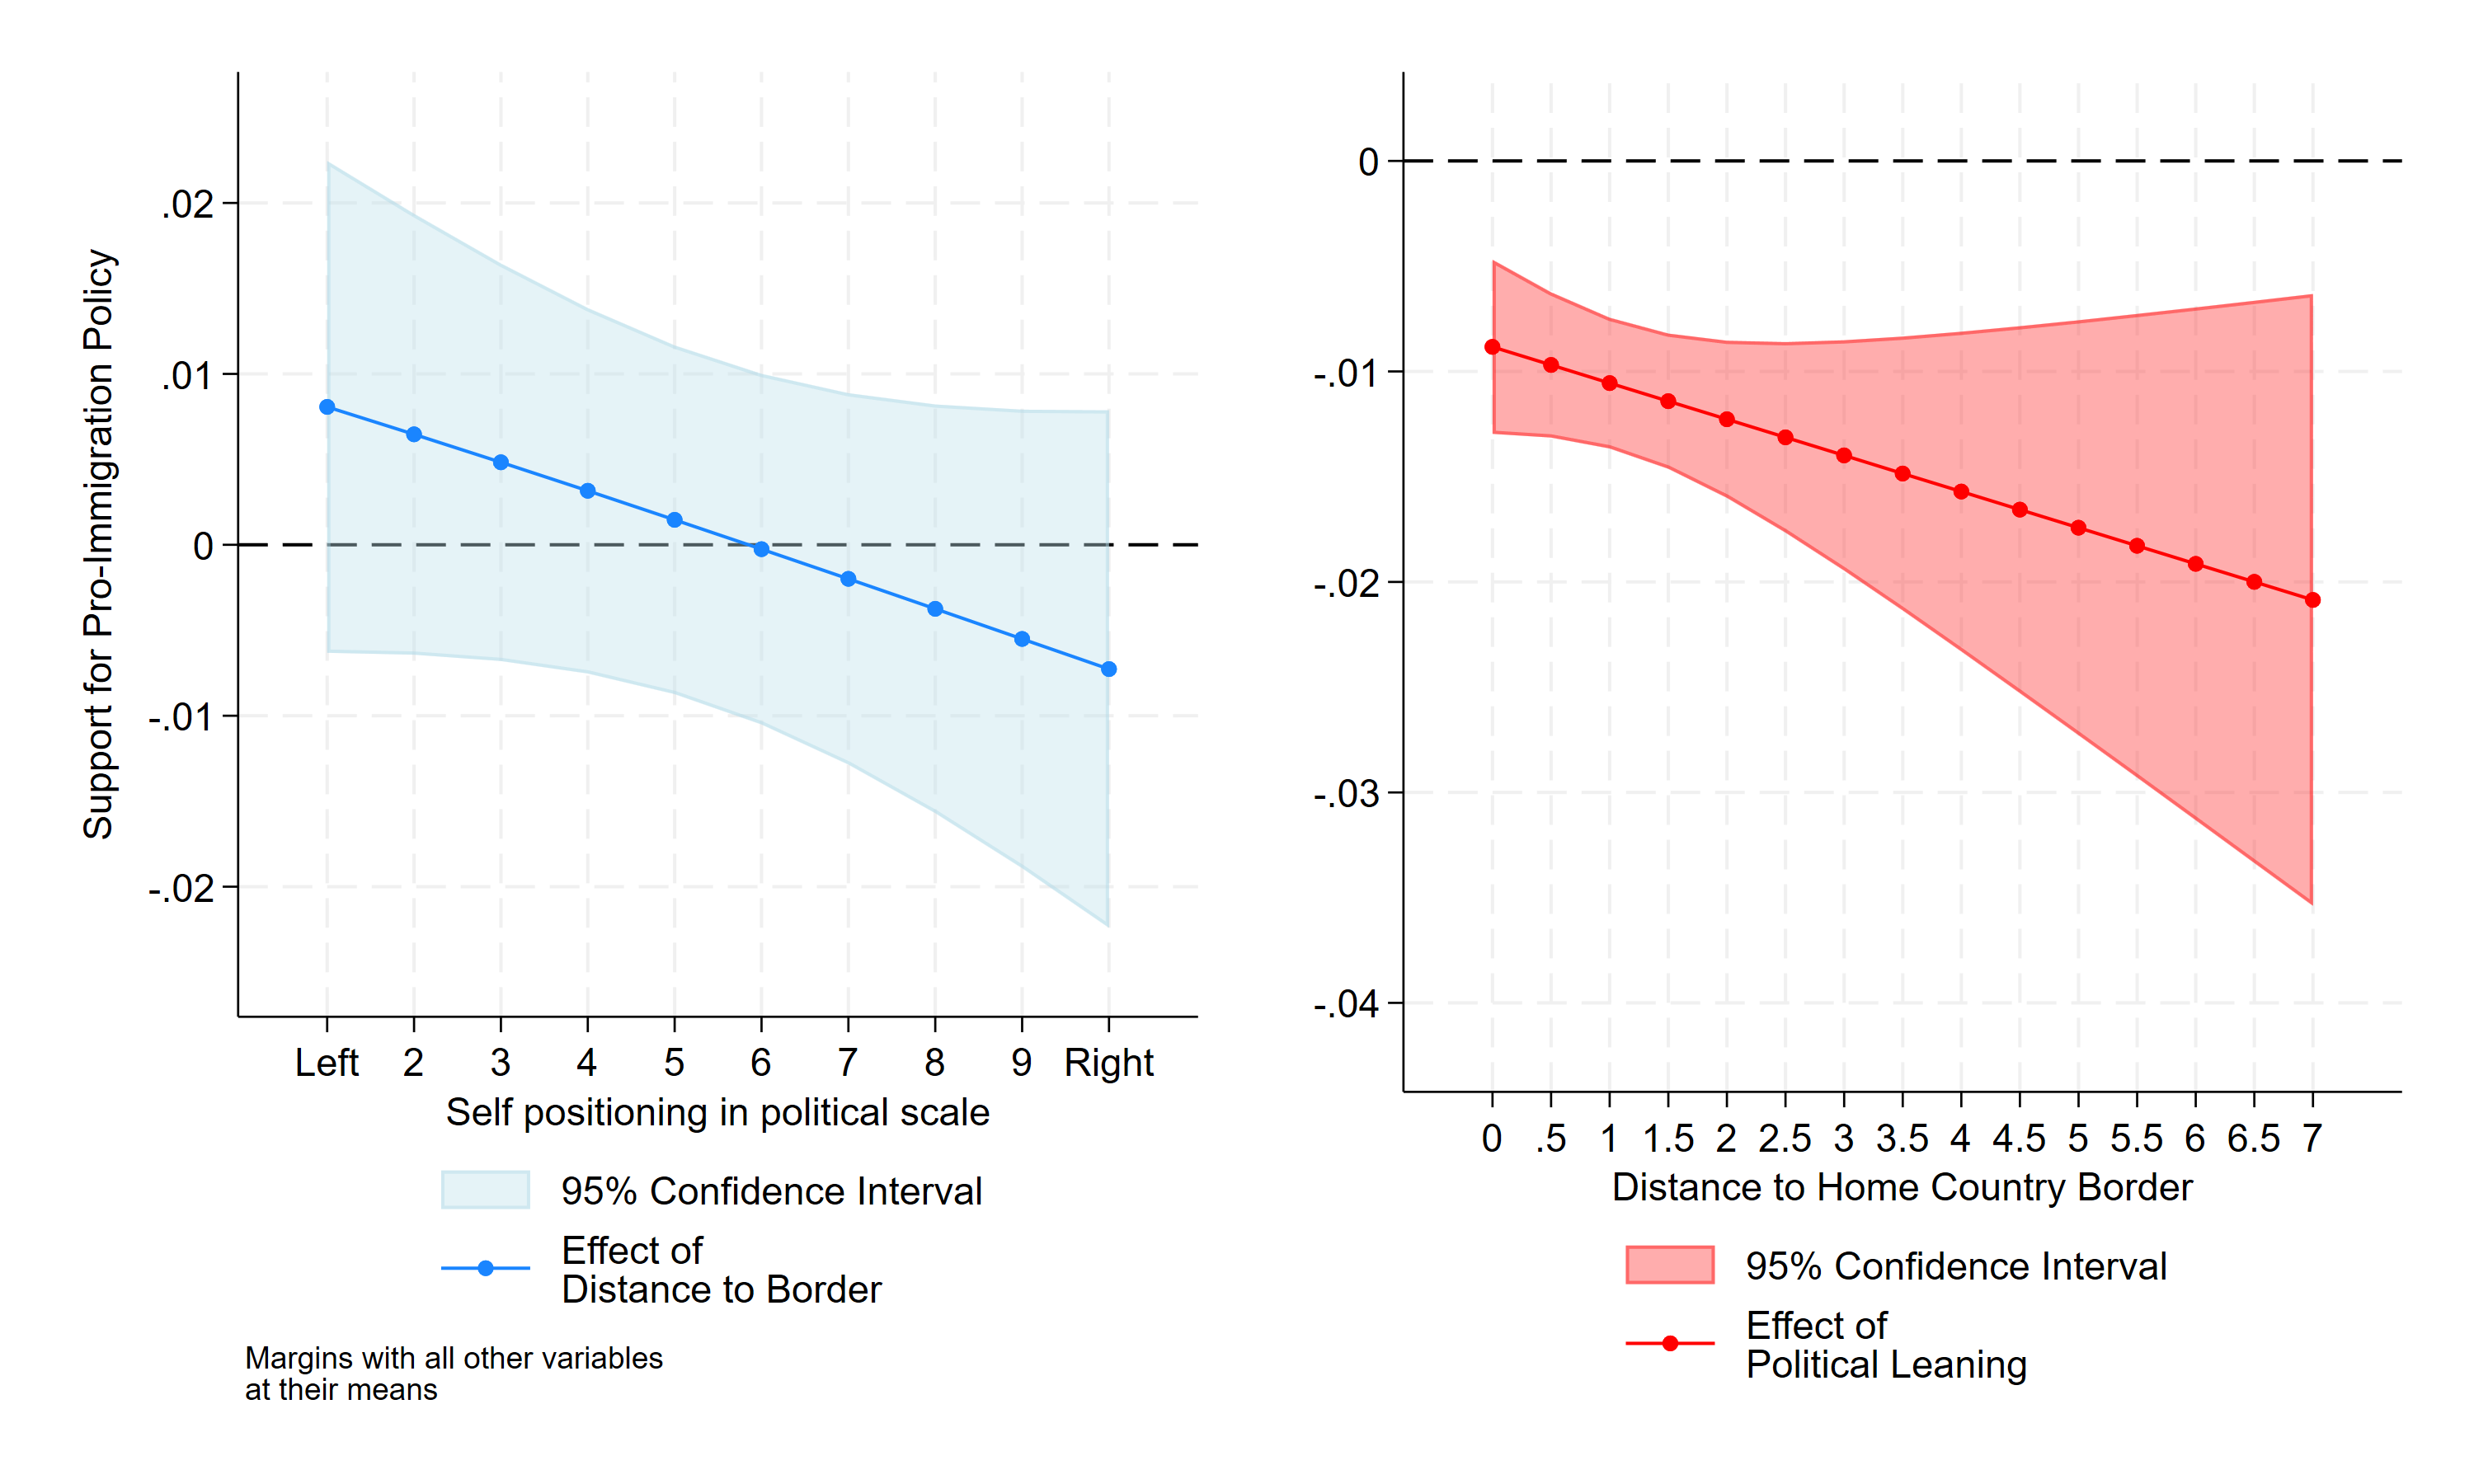
\includegraphics{figures/m5_policy_marginal_1.png} Figure 9 shows how as
border orientation becomes more controlling, the effect of conservatism
trends towards reduced opposition to migrants. Ultimately, as the latent
scale increases, the effect of ideology becomes increasingly muted,
showcasing a relative dominant role of border orientation in the
interaction given the null impact that ideology has on border
orientations' effect on public attitudes towards migrants. This provides
results opposite of Hypothesis 4, in which orientation should strengthen
the role of conservatism on opposition to migrants. This may suggest
that as policy becomes more in line with what strong conservatives may
want, ideology becomes a less salient determinant of opposition to
migrant now that conservative policy is reflected in the status quo.

\begin{figure}
\centering
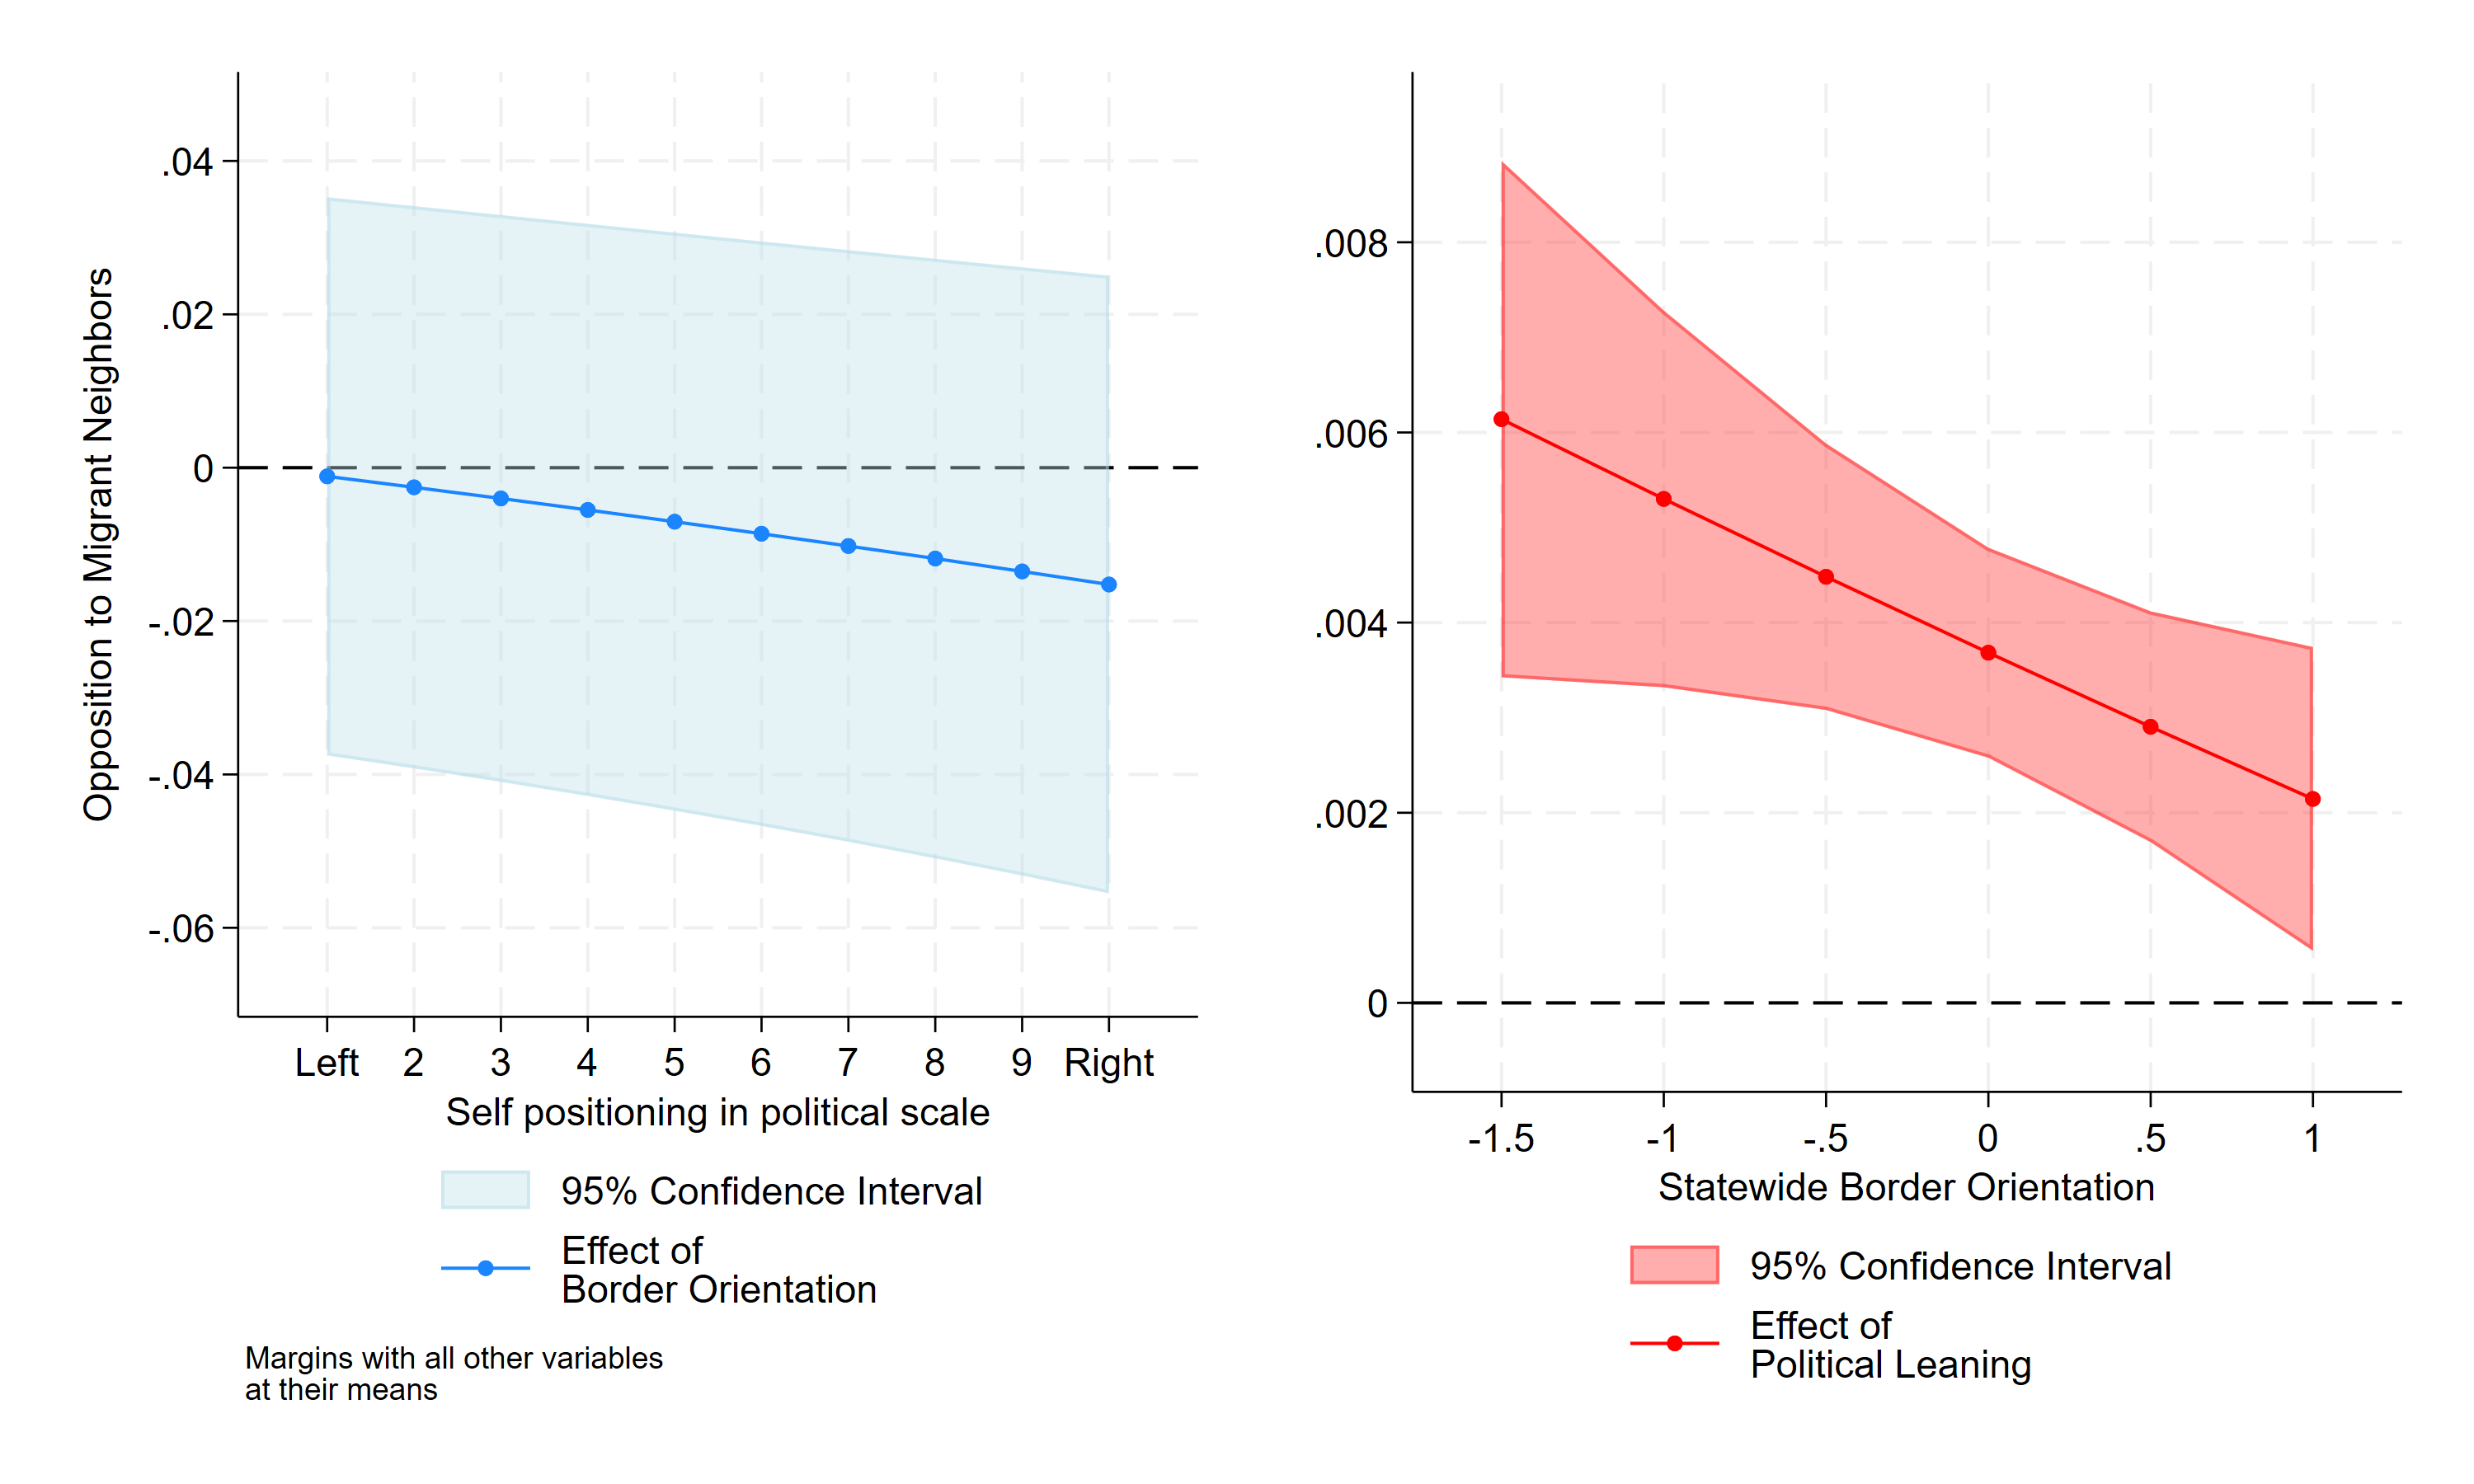
\includegraphics{figures/m6_marginal_1.png}
\caption{Figure 9: Testing H4 - Opposing Migrant Neighbors}
\end{figure}

\begin{figure}
\centering
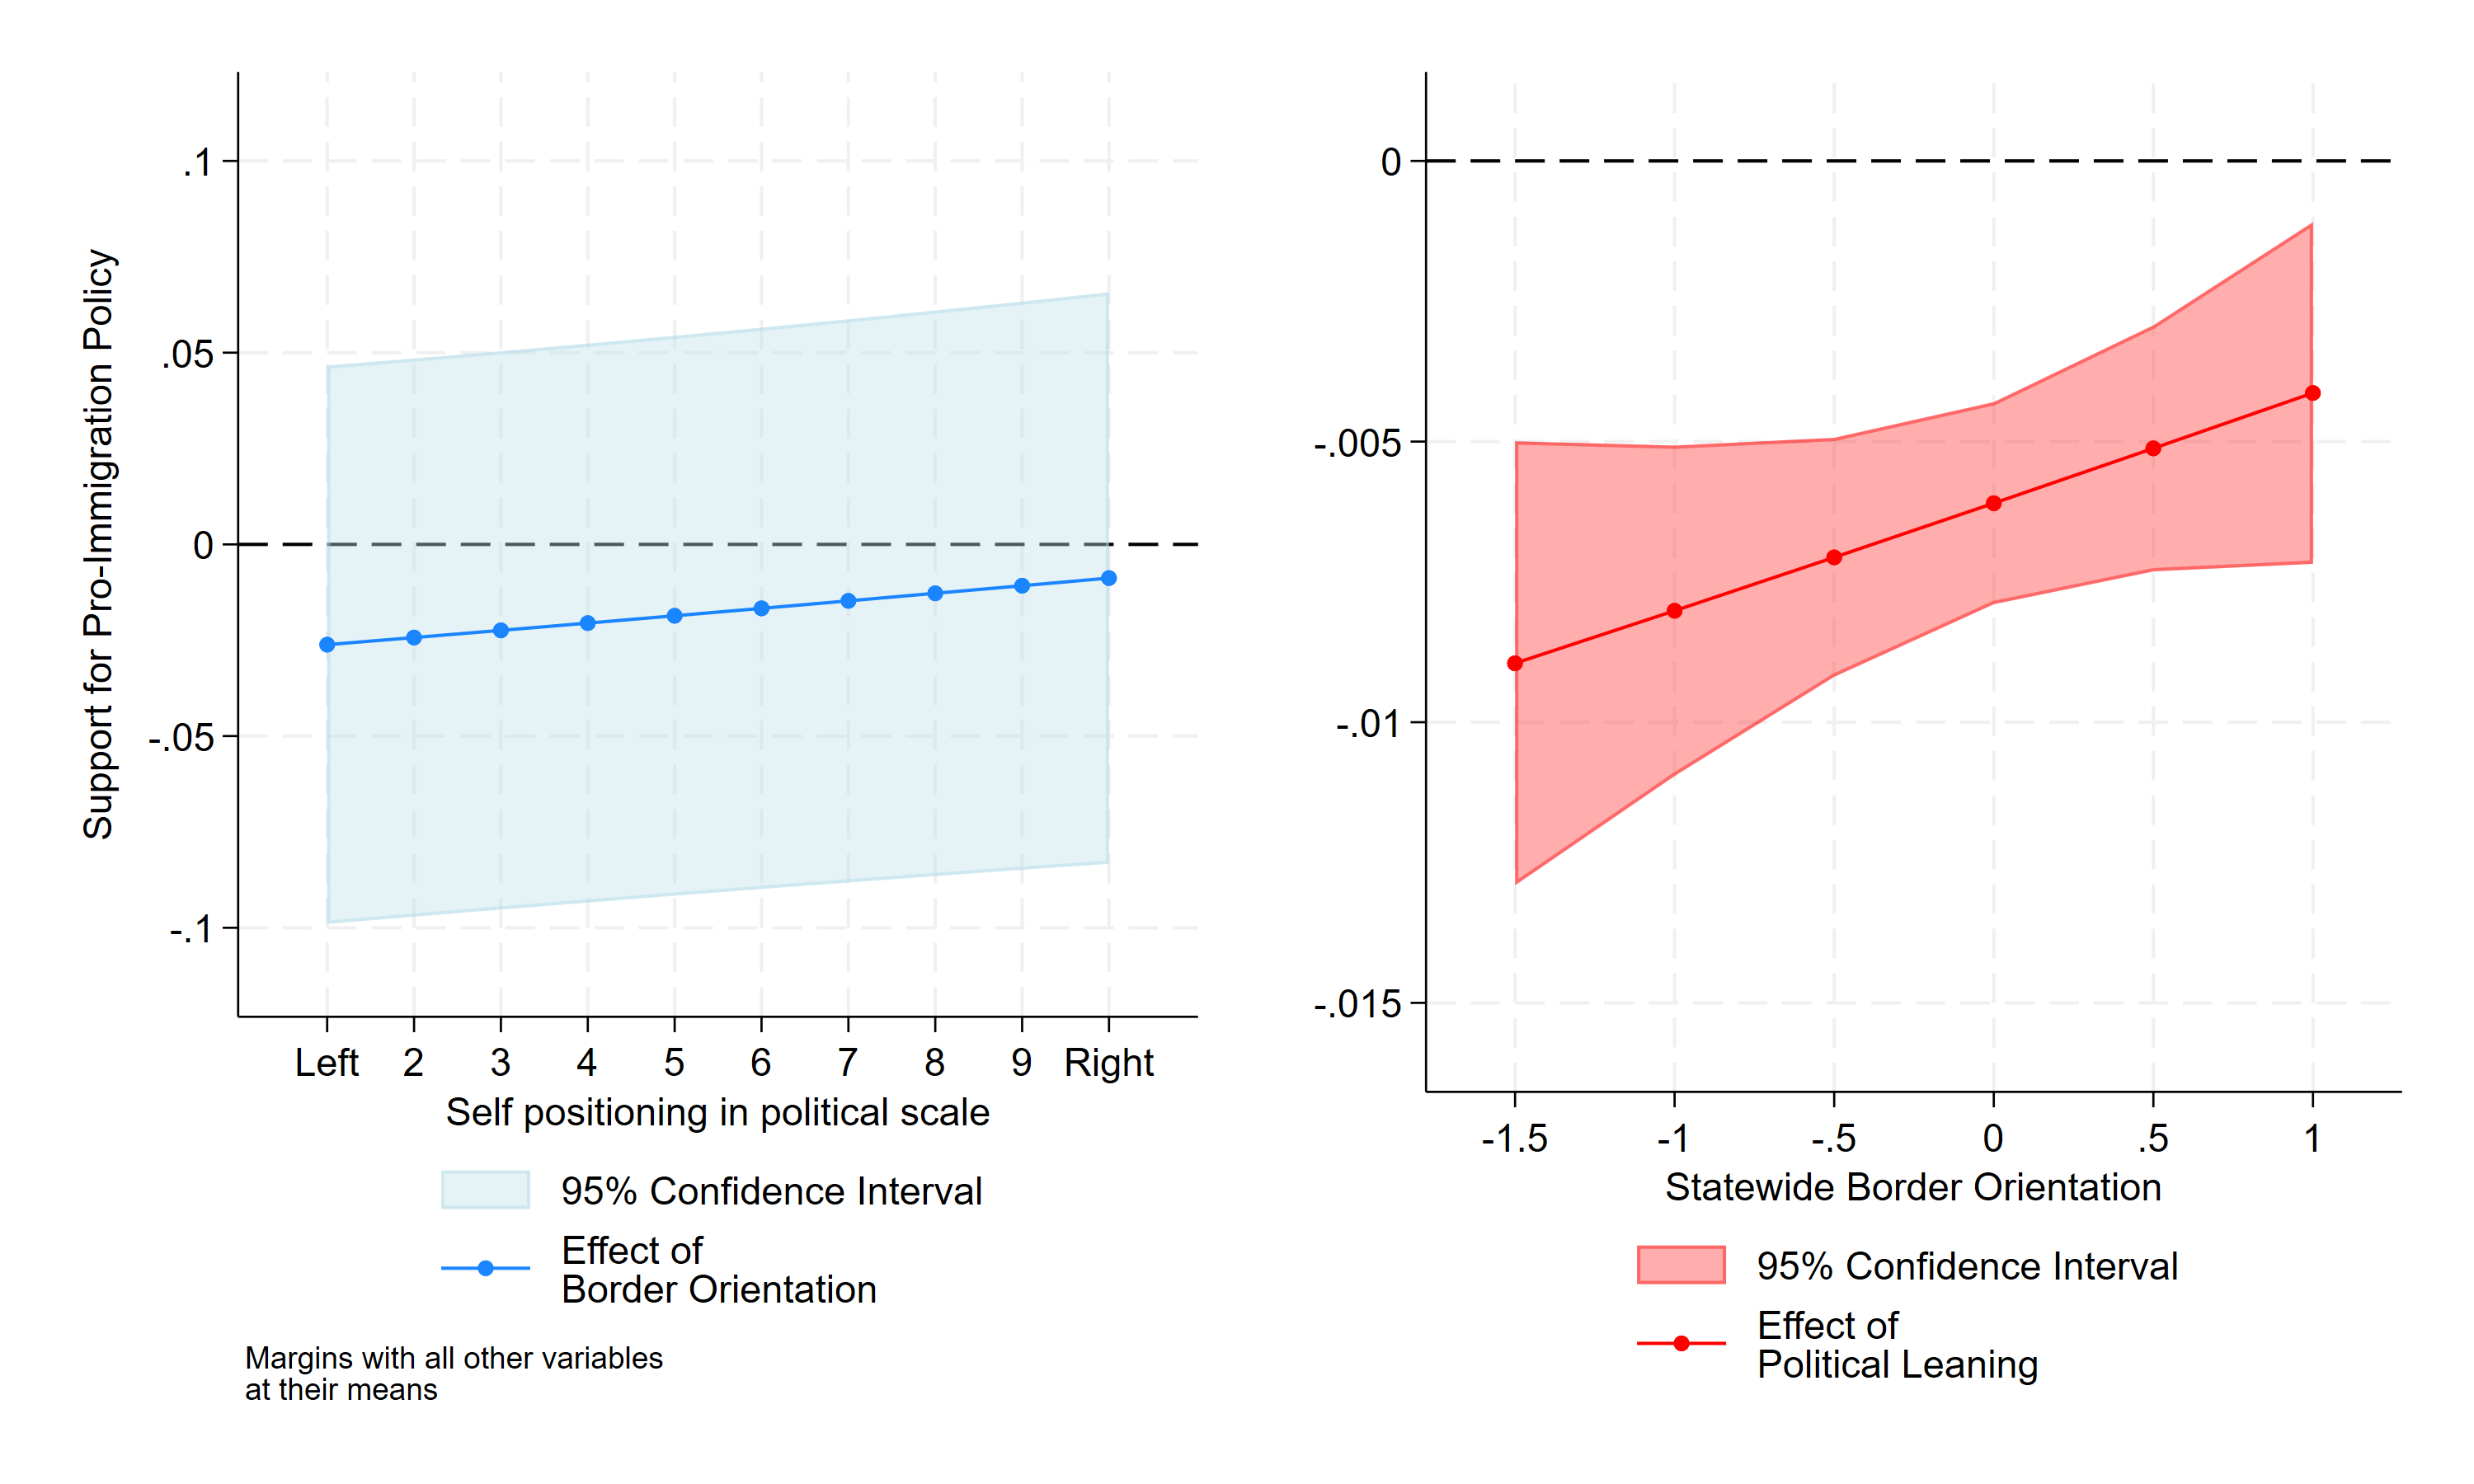
\includegraphics{figures/m6_policy_marginal_1.png}
\caption{Figure 10: Testing H4 - Pro-Immigrant Policy}
\end{figure}

\section{Discussion and Conclusion}\label{discussion-and-conclusion}

Ultimately, I find little or mixed evidence in favor of my hypotheses. I
find minimal evidence for higher levels of border fortifications
resulting in negative attitudes towards migrants or immigration policy,
and rather I find some evidence that police presence near the border may
result in improved attitudes towards migrants. Regardless of the little
evidence for Hypothesis 1, this research leads to next steps for the
literature on immigration attitudes. First, the significant findings for
the role of general trust in the public on immigration attitudes as well
as the negative impact of border police presence indicates support for
the idea of safety as a considerable influence on immigration, whether
it be narratives used by the government \citep{bajomi-lazar2019} or
events that occur within a country that increase the saliency of such
concerns \citep{young2018}. As such, perceptions of immigrant
criminality and the safety of residents from `bad actors' may be a
fruitful direction to continue exploring.

I also find minimal evidence for the role of distance playing a major
role in how border fortifications influence public opinion, but I do
find some evidence that respondents' distance to the border may alter
the effect of their political ideology on attitudes towards migrants and
immigration, albeit in the opposite direction as hypothesized. As
respondents live further from the border, the impact of increased
conservatism on opposition to migrants becomes increasingly muted.
However, as respondents live further from the border, increased levels
of conservatism result in a higher likelihood of opposing
pro-immigration policy. This provides some evidence in favor of the role
of intergroup theory, in which respondents with greater contact with
migrants or the border itself are more likely to support favorable
policies towards migrants, and less likely to be opposed to interacting
with migrants. I also find results in the opposite direction of
Hypothesis 4, where I find that as border fortifications shift to become
more controlling, ideology has a lower impact on opposition to migrants.

Future research could improve on these findings in multiple ways. First,
improving the matching or estimation procedure for attaining estimates
of respondents' distance to the border could help further confirm the
validity and robustness of the findings. As of now, the fuzzy matching
procedure provides some level of confidence that distances are
accurately assigned to respondents' districts, but further specification
may bolster confidence in the accuracy of the sample data further as
well as potentially improve the available sample size of the data.
Relatedly, using a single-case or small-n case design rather than a
large-n design may prove more fruitful for theory-testing. While the
results provide evidence on the general relationships between these key
variables, investigating a `most likely' case may help discern if these
(lack of) dynamics exists in at least some circumstances. A large
cross-national time-series sample such as the IVS may be fruitful for
general relationships, but given a lack of significance, further
investigation in a less generalizing sample may be a more accurate or
useful test of the theory.

\begin{verbatim}
As border fortifications continue to develop in the post-Cold War era [@carter2017], policymakers are likely to continue using narratives related to criminality or safety as justifications for their actions. Future research could investigate how such narratives impact respondents' levels of trust, and therefore make another empirical connection between state narratives, policymaker and elite conduct, and public opinion. Additionally, the role of ideology and immigration attitudes has been well studied. These findings continue to showcase this trend, but they further show that ideology is not necessarily independent of other contextual factors, especially factors that may be outside of the respondents' control and in the control of policymakers, like border policy.
\end{verbatim}

\subsection{Citations}\label{citations}




\newpage
\singlespacing 
\bibliography{publicopinioncitations.bib}

\end{document}